\chapter{Module Design and Implementation\label{ch:Module Design and Implementation}}
So far we have designed the software at the system level and learned background knowledge for implementation. In this chapter, we will design and implement each class.

\section{Main Window}
According to the requirements, we designed the main window as shown in Figure \ref{fig:Main Window}. The main window is not a unity as it seems to be. In fact, four classes are involved here: \textbf{RegisterManager}, which is the framework of the main window, \textbf{ChipNavigator}, \textbf{ChipEditorView} and \textbf{DocumentEditorView}. Their user interfaces are independently designed and compose the whole main window.

\begin{figure}[htb]
\centering
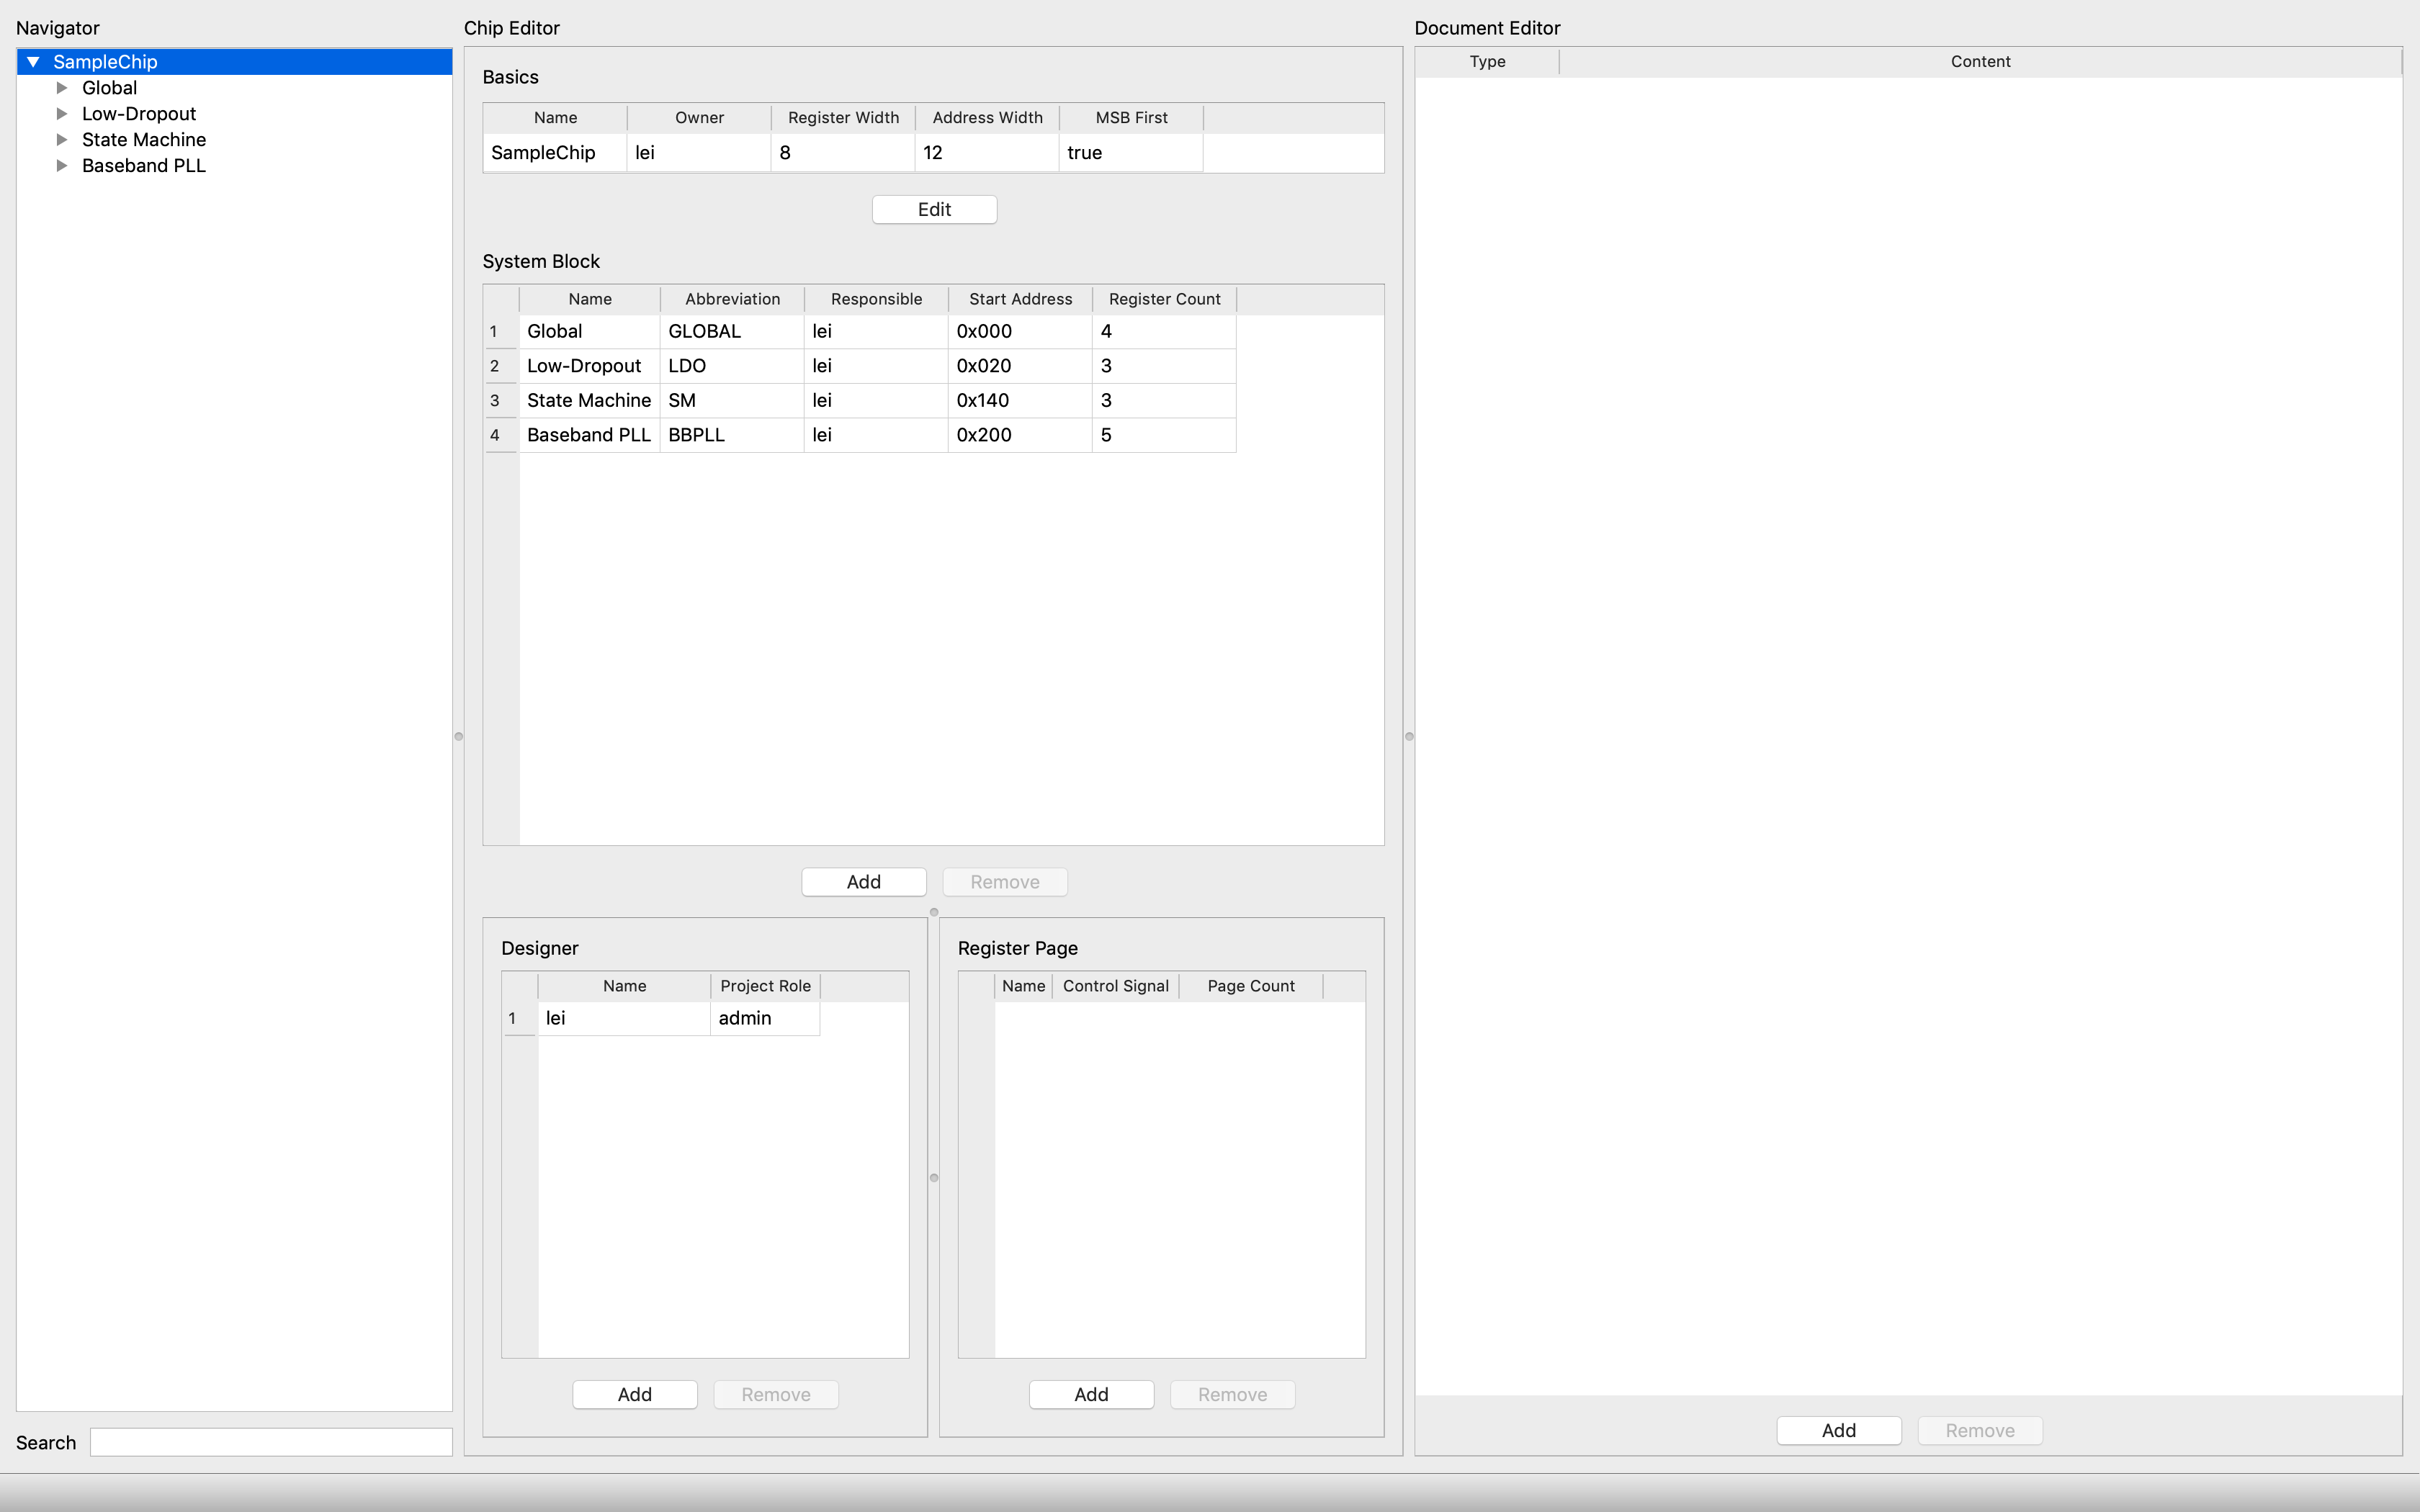
\includegraphics[width = \textwidth]{mainwindow}
\caption{Main Window\label{fig:Main Window}}
\end{figure}

We have described in the Chapter \ref{ch:Software Architecture Design} how these components work together. When the current item of the \textbf{ChipNavigator} changes, the \textbf{ChipEditorView} and the \textbf{DocumentEditorView} have to respond. To make this happen, we defined a slot function in the \textbf{ChipNavigator} to deal with the predefined \textbf{currentItemChanged()} signal of the tree widget. According to the level of the current tree widget item, we know whether it is the chip, a system block, a register, or a signal. Then, we defined signal functions for each level and emit them accordingly. The logic can be described by Code \ref{lst:Logic of Chip Navigation: Emission of Signals}.

\begin{minipage}{\linewidth}
\begin{lstlisting}[language=C++, caption={Logic of Chip Navigation: Emission of Signals\label{lst:Logic of Chip Navigation: Emission of Signals}}]
void  on_treeWidgetBlock_currentItemChanged(QTreeWidgetItem *current, QTreeWidgetItem *previous)
{
    if (level(current) == LEVEL::CHIP) 
        emit(chip_clicked());
    if (level(current) == LEVEL::BLOCK) 
        emit(block_clicked(get_block_id(current)));
    if (level(current) == LEVEL::REGISTER) 
        emit(register_clicked(get_block_id(current), get_register_id(current)));
    if (level(current) == LEVEL::SIGNAL) 
        emit(signal_clicked(get_block_id(current), get_signal_id(current)));
}
\end{lstlisting}
\end{minipage}

To take care of the signal, we defined slot functions in the \textbf{RegisterManager} class (see Code \ref{lst:Logic of Chip Navigation: Declarations of Slot Functions}) and connect them to corresponding signals. In the slot functions, we first update the current block, register and signal ID. Then, we reset the document level. We pass the IDs to the \textbf{ChipEditorView} and \textbf{DocumentEditorView}, then let them display documents and chip information respectively. See Code \ref{lst:Logic of Chip Navigation: Definitions of Slot Functions}.

\begin{lstlisting}[language=C++, caption={Logic of Chip Navigation: Declarations of Slot Functions\label{lst:Logic of Chip Navigation: Declarations of Slot Functions}}]
// register_manager.h
void on_chipNavigator_chip_clicked();
void on_chipNavigator_block_clicked(QString block_id);
void on_chipNavigator_register_clicked(QString block_id, 
        QString reg_id);
void on_chipNavigator_signal_clicked(QString block_id,
        QString sig_id);
\end{lstlisting}

\begin{lstlisting}[language=C++, caption={Logic of Chip Navigation: Definitions of Slot Functions\label{lst:Logic of Chip Navigation: Definitions of Slot Functions}}]
// register_manager.cpp
void RegisterManager::on_chipNavigator_register_clicked(QString block_id, QString reg_id)
{
    ui->docEditorView->set_doc_level(LEVEL::REGISTER);
    ui->docEditorView->set_block_id(block_id);
    ui->docEditorView->set_register_id(reg_id);
    if (ui->frameDoc->isVisible() && ui->actionDocEditor->isChecked()) 
        ui->docEditorView->display_documents();

    ui->chipEditorView->set_block_id(block_id);
    if (ui->frameChipEditor->isVisible()) 
        ui->chipEditorView->display_system_level_info(reg_id);
    current_block_id_ = block_id;
    current_reg_id_ = reg_id;
    current_sig_id_ = "";
}
\end{lstlisting}

We can edit the chip in the \textbf{ChipEditorView} by editing the chip name, adding, editing or removing system blocks, registers, signals, signal-register mappings and so on. In these cases, the chip navigator have to be updated. Similarly, we define signals in the \textbf{ChipEditorView} as in Code \ref{lst:Signals for Updating the Chip Navigator}, and corresponding slot functions in the \textbf{RegisterManager}. When the chip is edited, a certain signal is emitted and information is passed to the corresponding slot function in the \textbf{RegisterManager}. In the slot function, a certain function of the chip navigator is called to update the tree widget.

\begin{lstlisting}[language=C++, caption={Signals for Updating the Chip Navigator\label{lst:Signals for Updating the Chip Navigator}}]
// chip_editor_view.h
void chip_basics_edited(QString chip_name, 
                  QString chip_owner, 
                  QString chip_owner_id, 
                  int register_width, 
                  int address_width, 
                  bool msb_first);
void block_added(QString block_id, 
                  QString block_name, 
                  QString block_abbr, 
                  QString responsible);
void block_removed(int row);
void block_modified(int row, 
                  QString block_name, 
                  QString block_abbr, 
                  QString responsible);
void block_order_exchanged(int from, int to);
void to_refresh_block(); 
\end{lstlisting}

The boundaries between the \textbf{ChipNavigator}, \textbf{ChipEditorView} and \textbf{DocumentEditorView} are adjustable. Users can also switch on or off the \textbf{ChipEditorView} or the \textbf{DocumentEditorView}. 

We designed a menu bar for the main window. There are four menus as follows, each containing a number of menu entries, or actions.
\begin{itemize}
\item \textbf{User Menu} \\
\textbf{User Management}: to open a \textbf{UserManagementDialog} in which users can add or remove users. It is only accessible to database admins. \\
\textbf{Change Password}: to open a \textbf{ChangePasswordDialog} for users to change their password. \\
\textbf{Log Out}: to log out of the current user account and to log in with another one. 
\item \textbf{Chip} \\
\textbf{New Chip}: to open an \textbf{EditChipDialog} to create a new chip. \\
\textbf{New Chip From}: to create a new chip from an existing one. \\
\textbf{Open Chip}: to open an \textbf{OpenChipDialog} and open the selected chip. \\
\textbf{Close Chip}: to close the current chip and clear everything in the \textbf{ChipNavigator}, \textbf{ChipEditorView} and \textbf{DocumentEditorView}. \\
\textbf{Naming}: to open a \textbf{NamingTemplateDialog} to display the namings for registers or signals. \\
\textbf{Resources Base Dir}: to open a \textbf{ResourcesBaseDirDialog} in which users can specify the base directory where resources such as figures are located. \\
\textbf{Freeze/Unfreeze}: to freeze or unfreeze the current chip. \\
\textbf{Chip Management}: to open an \textbf{OpenChipDialog} and configure it to the management mode. Users can add or remove chips. It is only accessible to database admins. 
\item \textbf{Export} \\
\textbf{SPI Source Code}: to open an \textbf{SPIGenerationDialog} and generate the SPI interface. \\
\textbf{Document}: to open an \textbf{DocumentGenerationDialog} and generate the documentation. 
\item \textbf{View} \\
\textbf{Chip Editor}: to enable or disable the \textbf{ChipEditorView}. \\
\textbf{Document Editor}: to enable the \textbf{Document Editor} page of the \textbf{DocumentEditorView}. \\
\textbf{Document Preview}: to enable the \textbf{Document Preview} page of the \textbf{DocumentEditorView}. The \textbf{Document Editor} and \textbf{Document Preview} actions are exclusively checkable. 
\end{itemize}

\subsection{ChipNavigator}
We have described the logic of the main window and its interaction with the \textbf{ChipNavigator}, the \textbf{ChipEditorView} and the \textbf{DocumentEditorView}. The \textbf{ChipNavigator} is quite simple. According to requirements, the structure of the chip is represented with a tree widget of four levels: CHIP-BLOCK-REGISTER-SIGNAL. The root of the tree is the chip level, with its children being system blocks. Under each system block are registers. The children of each register are those signals mapped to it.

We implemented a search mechanism which might be very beneficial especially when the chip is complex. The users can simply type in the pattern to search, and the tree widget will highlight those components matching that pattern and make others invisible. The search process is written in a single \textbf{search()} function. Whenever the input pattern changes, the \textbf{search()} function will be executed in response to the \textbf{textChanged()} signal from the tree widget. Figure \ref{fig:Chip Navigator: Search Example} shows an example of the search process.

\begin{figure}[htb]
\centering
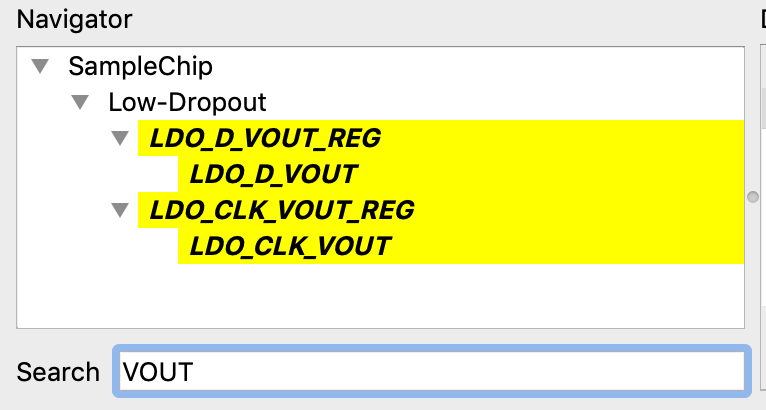
\includegraphics[width =0.5 \textwidth]{searchtree}
\caption{Chip Navigator: Search Example\label{fig:Chip Navigator: Search Example}}
\end{figure}

\subsection{Chip Editor View}
The \textbf{ChipEditorView} is one of the three major components of the main window. It displays information about the chip and provides entrance to dialogs for editing the chip. According to the requirements, we designed the \textbf{ChipEditorView} as in Figure \ref{fig:Chip Editor: Signal Tab} and \ref{fig:Chip Editor: Register Tab}.

\begin{figure}[htbp]
\centering
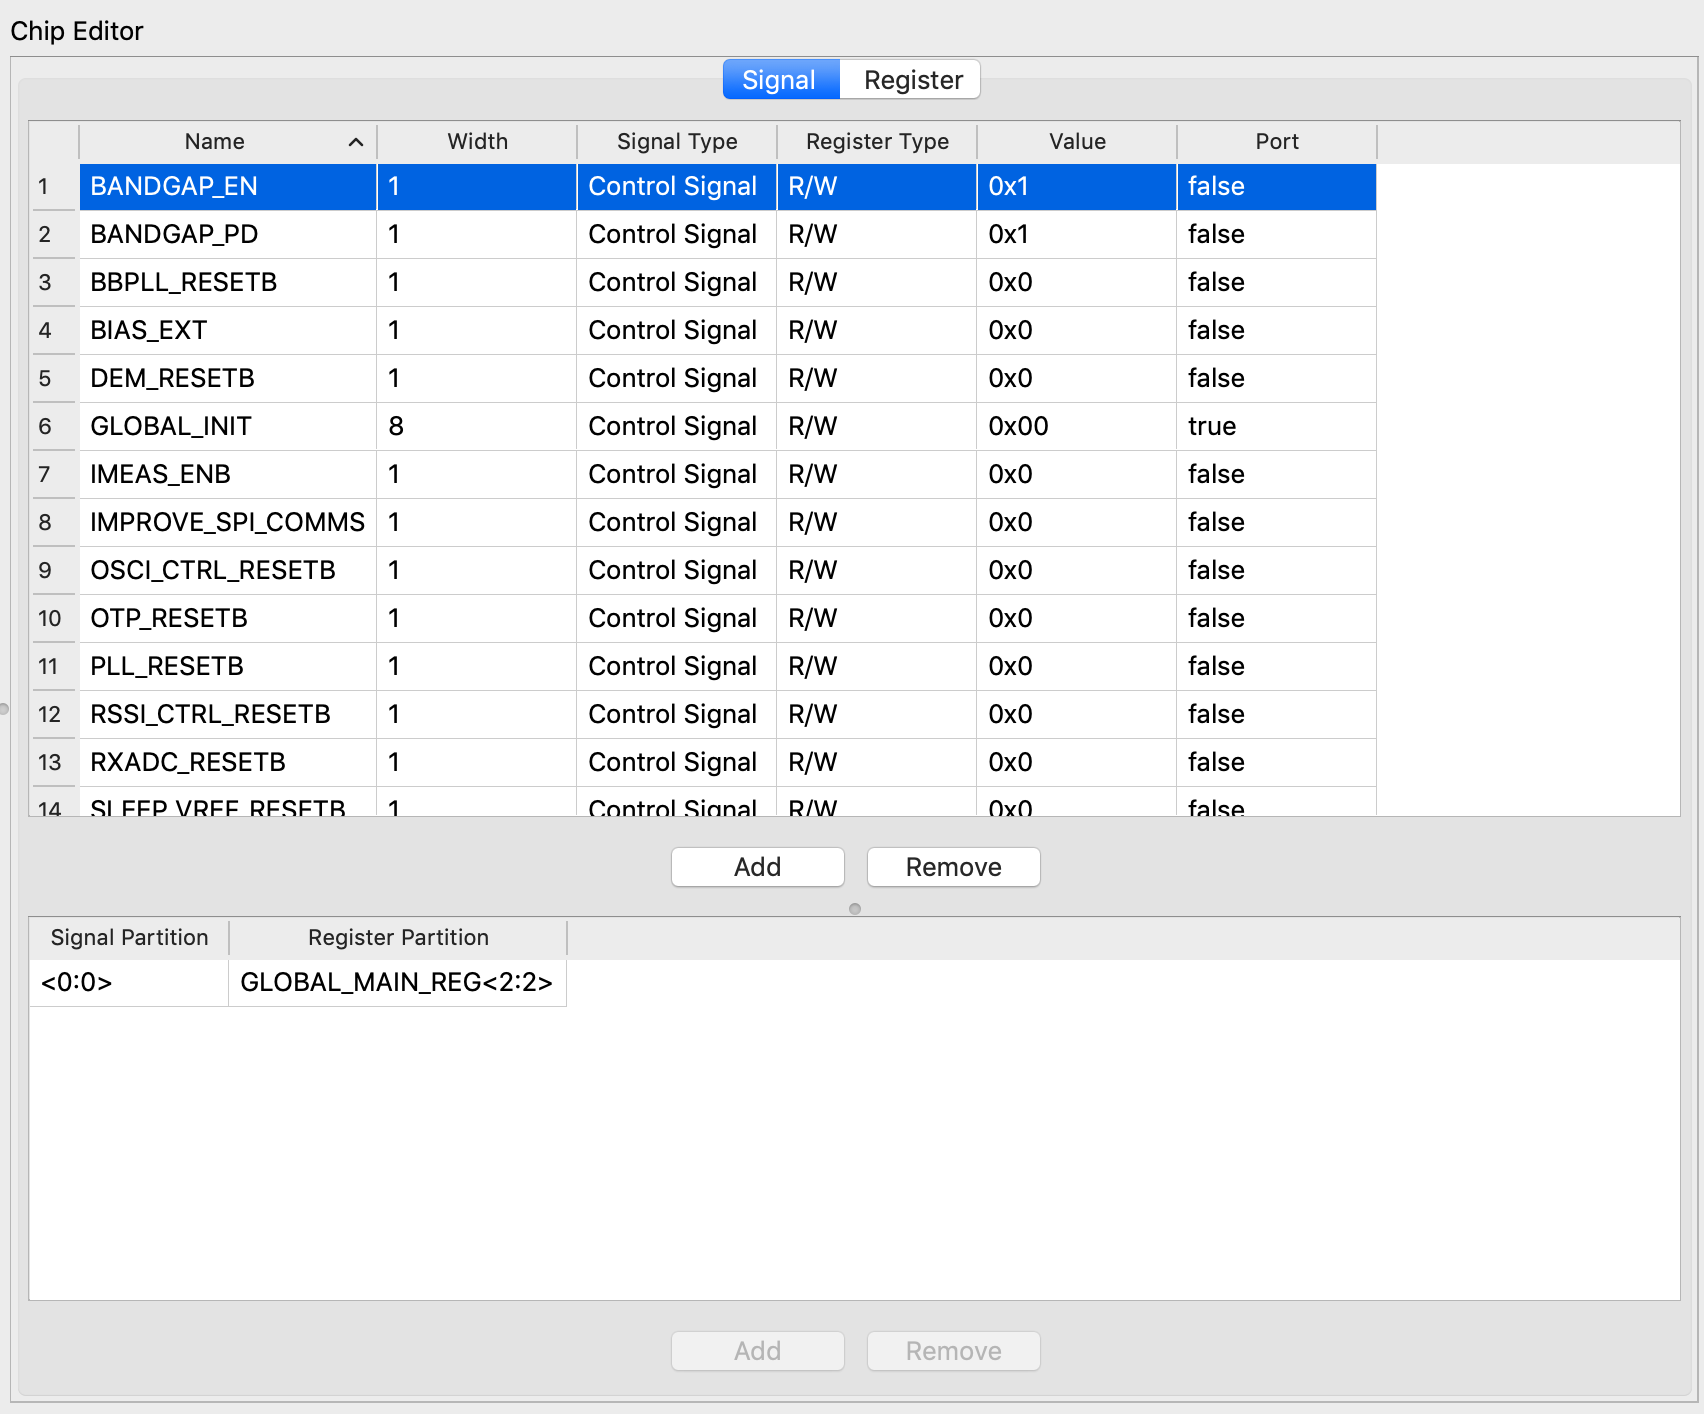
\includegraphics[width = \textwidth]{signalview}
\caption{Chip Editor: Signal Tab\label{fig:Chip Editor: Signal Tab}}
\end{figure}

\begin{figure}[htbp]
\centering
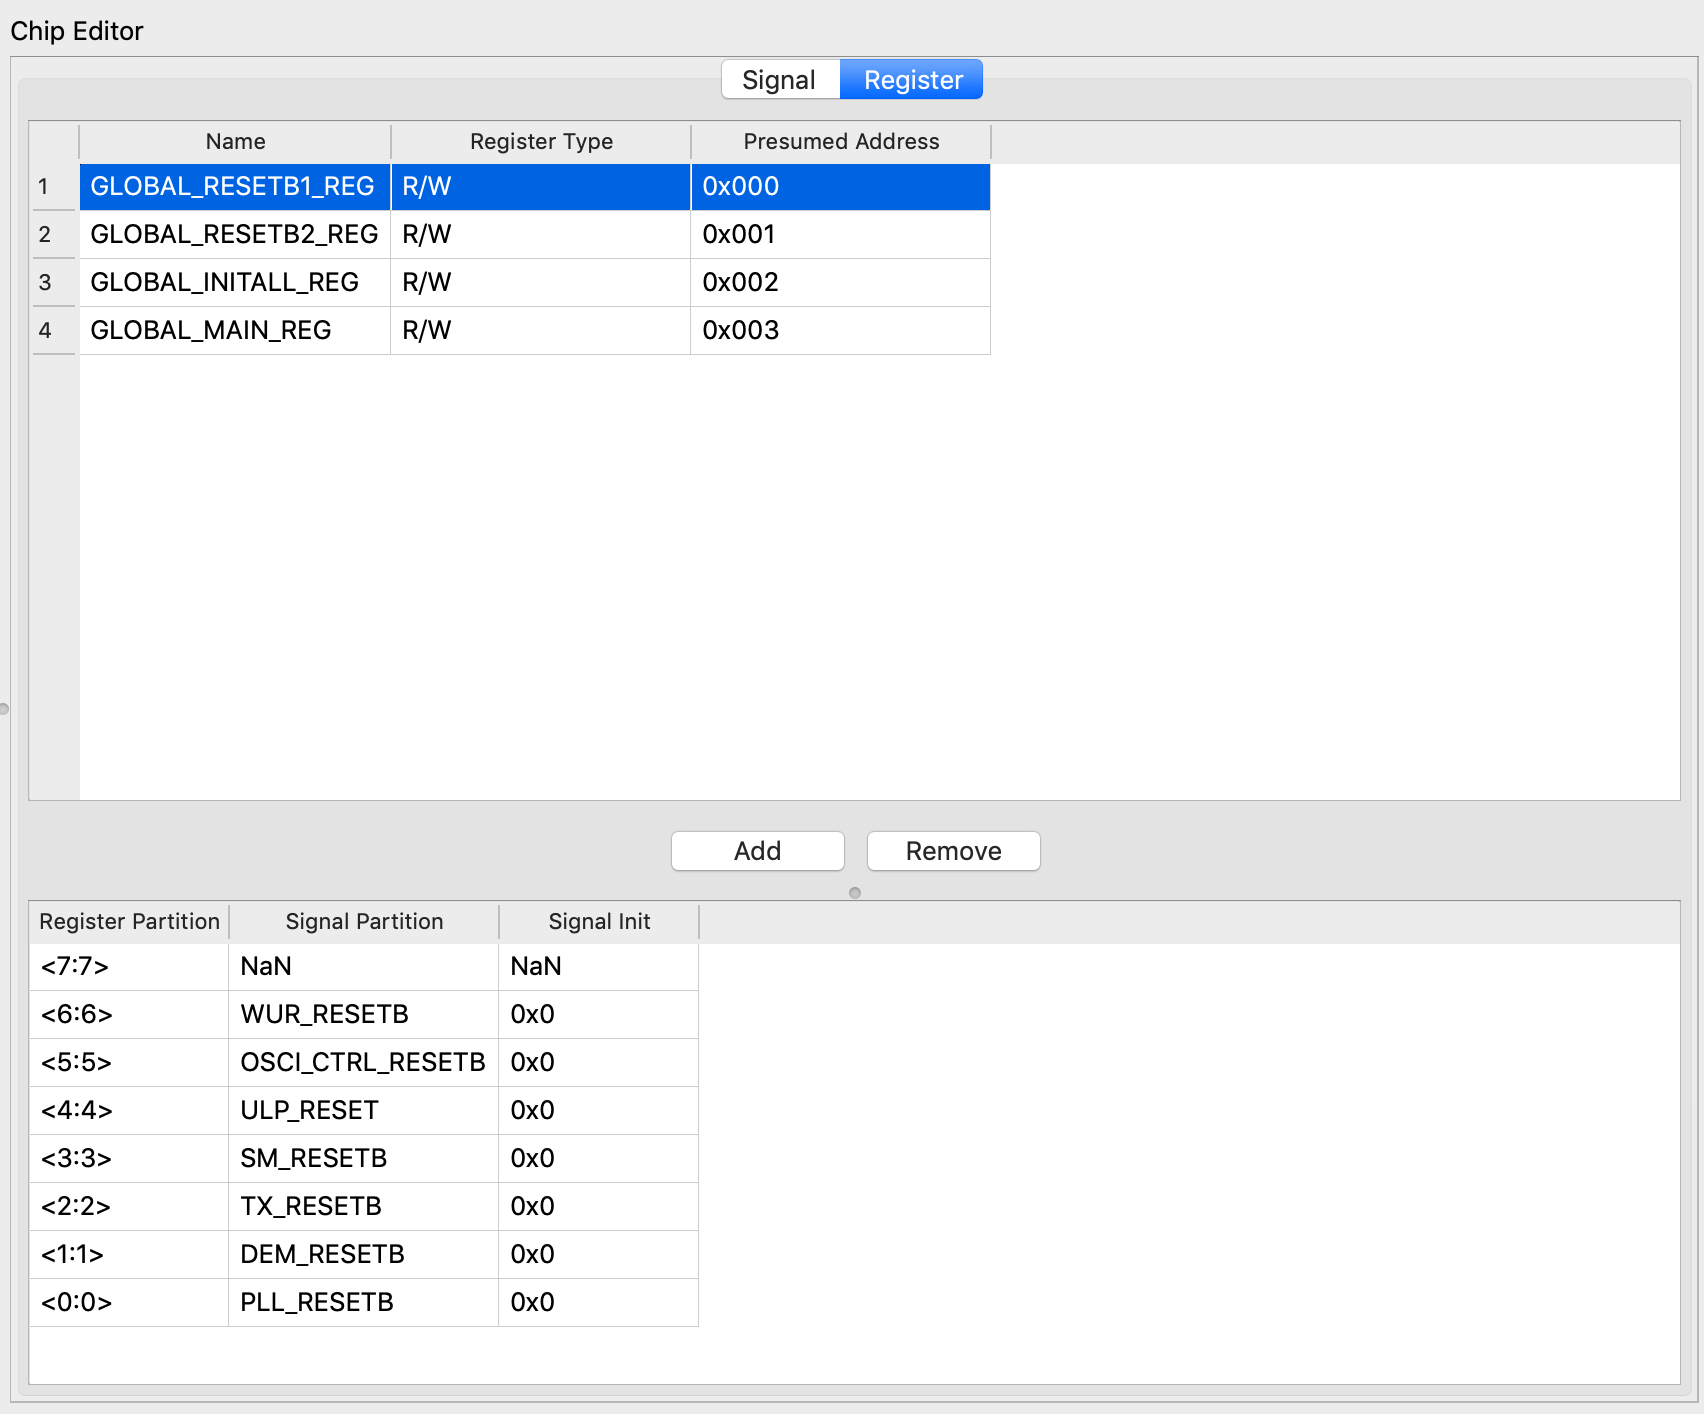
\includegraphics[width = \textwidth]{registerview}
\caption{Chip Editor: Register Tab\label{fig:Chip Editor: Register Tab}}
\end{figure}

Whether the chip level or the system level page is displayed depends on the current item of the navigator. If it is the root of the tree widget, then the \textbf{RegisterManager} class will call the \textbf{display\_chip\_level\_info()} function of the \textbf{ChipEditorView}, otherwise \textbf{display\_system\_level\_info(register\_id, signal\_id)} is called. If the current item is a register, then its \textbf{register\_id} will be passed to the function and \textbf{signal\_id} will be null. Likewise, if the item is a signal, then \textbf{register\_id} will be null. Depending on whether \textbf{register\_id} or \textbf{signal\_id} is null, the \textbf{ChipEditorView} will display the register page or the signal page, and set the selected register or signal in the register or the signal table as active. If the current item is a block, both \textbf{register\_id} and \textbf{signal\_id} are null, and the \textbf{ChipEditorView} simply displays the current page. This process can be described with the following simplified Code \ref{lst:Logic of Displaying System Level Information}.

\begin{lstlisting}[language=C++, caption={Logic of Displaying System Level Information}\label{lst:Logic of Displaying System Level Information}]
// chip_editor_view.cpp
void ChipEditorView::display_system_level_info(const QString& reg_id, const QString& sig_id)
{
    // set to system level page
    ui->stackedWidgetChipEditor->setCurrentIndex(1);

    // set to register or signal page
    if (sig_id != "") ui->tabWidget->setCurrentIndex(0);
    else if (reg_id != "") ui->tabWidget->setCurrentIndex(1);

    // display either signals or registers
    if (ui->tabWidget->currentIndex() == 0) display_signals();
    else display_registers();
    
    // set current signal as active
    if (sig_id != "")
    {
        for (int row = 0; row < ui->tableSignal->rowCount(); row++)
            if (sig_id == ui->tableSignal->item(row, 0)->text())
            {
                ui->tableSignal->setCurrentCell(row, 0);
                break;
            }
    }
    // set current register as active
    else if (reg_id != "")
    {
        for (int row = 0; row < ui->tableRegister->rowCount(); row++)
            if (reg_id == ui->tableRegister->item(row, 0)->text())
            {
                ui->tableRegister->setCurrentCell(row, 0);
                break;
            }
    }
}
\end{lstlisting}

To add a system block, register, signal or a signal-register mapping we provide a push button under each table. After a click on the button a dialog of the corresponding class will be created and open. To remove an existing item we can click on the \textbf{Remove} buttons leading to execution of a corresponding slot function. The function will first remove the system block, register etc. in the database, then remove it from the table. To edit an existing system block, register or signal, we can double click the table entry. The \textbf{cellDoubleClicked()} signal will then be emitted. We write corresponding slot functions to help us edit the items. The logic is actually very similar to adding a new item. A corresponding dialog will open, but it will be initialized with data related to that item. The dialogs will be discussed in the Section \ref{sec:Chip and Document Editor Dialogs}. 

For users' convenience, we designed a right-click context menu containing an \textbf{Edit}, \textbf{Remove} and \textbf{Add} action. Users do not have to click on the push buttons below each table. The menu also contains a \textbf{Refresh} action, which allows for reloading data from the database and refreshing the table. Once we right-click on the tables, a \textbf{customContextMenuRequested()} signal will be triggered. A slot function is then called to display the context menu in response to the signal.

\subsection{Document Editor View}
The \textbf{DocumentEditorView} shown in Figure \ref{fig:Document Editor View} is another central component of the software. It displays document items and provides functionality for editing them. According to the requirements, it should contain a table widget showing all document items of the current item on the chip navigator. At the bottom of the \textbf{DocumentEditorView} there is an editor "dialog" in which we can add or edit a document. It is an instance of the \textbf{EditDocumentDialog} class, which is not a real dialog though, but a subclass of the generic \textbf{QWidget}. This is because the \textbf{QDialog} cannot be a child widget of another Qt widget. The dialog can be switched on or off. Like the \textbf{ChipEditorView}, we can add or edit document items by clicking on the \textbf{Add} button below or double clicking a table entry. The editing dialog will then open. If we have finished editing and want to save the document, we click on the \textbf{Ok} button. The document will be saved to the database and the table above will be updated. Then, the editing area will be switched off. If we want to abandon the document we are editing, simply click on the \textbf{Cancel} button. 

\begin{figure}[htb]
\centering
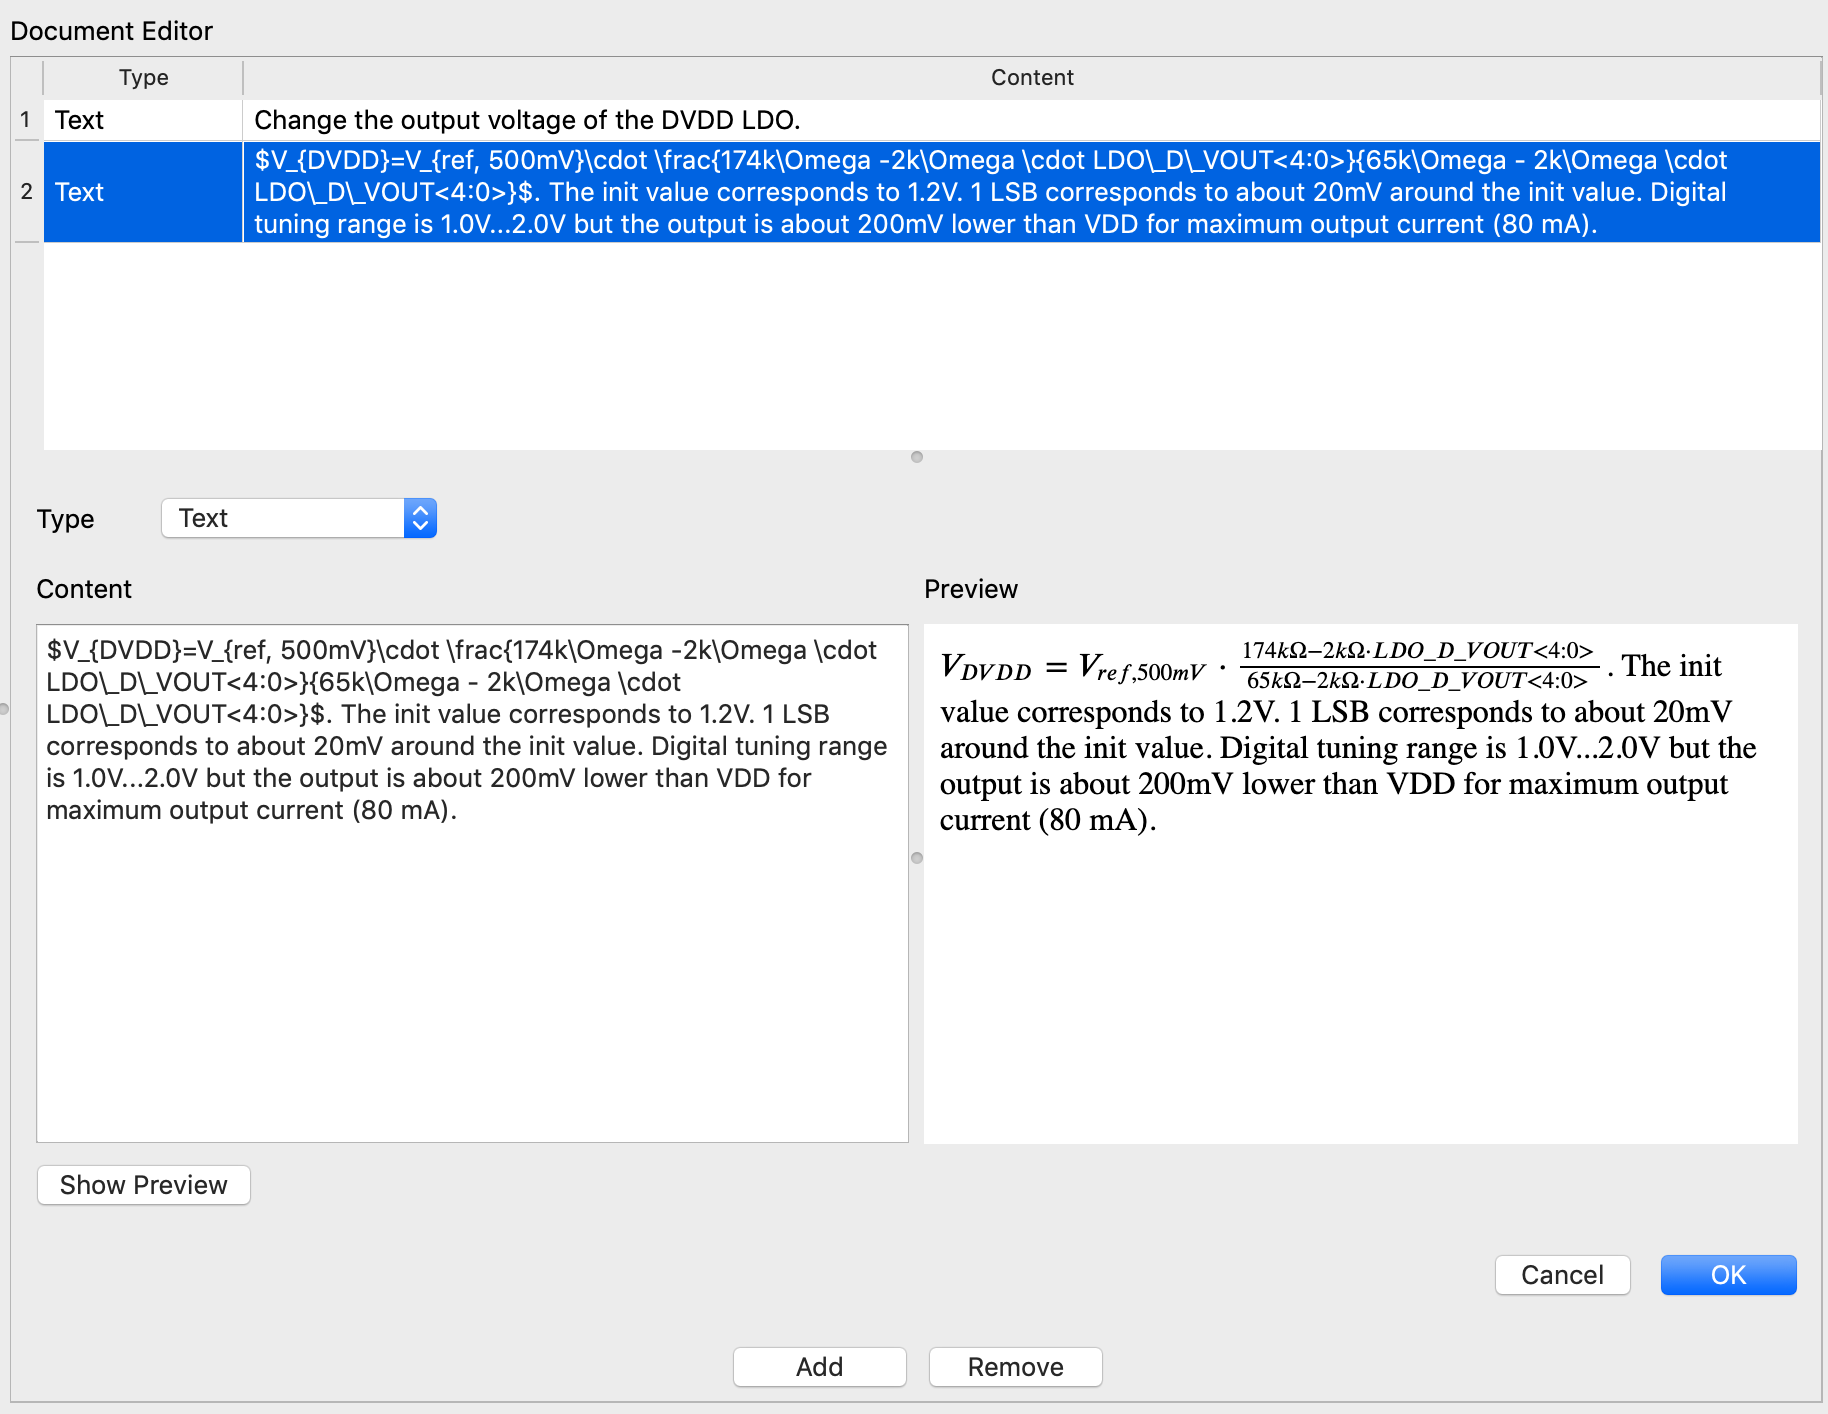
\includegraphics[width = \textwidth]{documentview}
\caption{Document Editor View\label{fig:Document Editor View}}
\end{figure}

Apart from the \textbf{Add}, \textbf{Remove} and \textbf{Edit} functions, we provided a copy and paste mechanism, which might be very useful for documentation editing. To achieve this, we maintain a member variable \textbf{copied\_} of type \textbf{QString}. When we copy a document, the corresponding document type ID, document type, and the content to copy will be concatenated by a special delimiter and then be stored in this \textbf{copied\_} variable. When we paste the copied content, the \textbf{copied\_} variable will be parsed to fetch the document type ID, document type, and the content to paste. With this information, we can create a new entry in the document table and store this document to the database.

\section{Chip and Document Editor Dialogs\label{sec:Chip and Document Editor Dialogs}}
To edit chip components and document items, we have to design different dialogs encapsulating both UI and business logics. These dialogs are named after \textbf{EditSomethingDialog}, such as \textbf{EditChipDialog} and \textbf{EditSignalDialog}. They are defined following the framework in Code \ref{lst:Framework for Chip and Document Editor Dialog Classes}.

\begin{lstlisting}[language=C++, caption={Framework for Chip and Document Editor Dialog Classes\label{lst:Framework for Chip and Document Editor Dialog Classes}}]
// edit_something_dialog.h
class EditSomethingDialog : public QDialog
{
    Q_OBJECT

public:
    explicit EditSomethingDialog(QWidget *parent = nullptr);
    explicit EditSomethingDialog(QString something_id, bool enabled, QWidget *parent = nullptr);
    // other construction functions
    ~EditSomethingDialog();
    QString get_something_id();
    // Other public functions
    
    bool add_something();
    bool edit_something();

private:
    bool setup_ui();
    void accept(); // override QDialog::accept()
    bool sanity_check();
    /*
     Things to check
    */
    // Other private functions

    Ui::EditSomethingDialog *ui;
    const bool enabled_;
    const DIALOG_MODE mode_;
    QString something_id_;
    // Other private member variables 
};
\end{lstlisting}

The class has at least two construction functions, one for adding, the other for editing something. The \textbf{DIALOG\_MODE} \textbf{mode\_} will correspondingly set to \textbf{ADD} or \textbf{EDIT}. Upon construction the dialog first sets up the UI by calling the \textbf{setup\_ui()} function. If the dialog is constructed in the \textbf{EDIT} mode, it will pass the ID to the dialog and fill in the existing data into the widgets. Also, there is a parameter called \textbf{enabled}. If it is false, then the UI components will be disabled so users cannot put in anything to the dialog. Otherwise, users give their inputs to the dialog and click on the \textbf{Ok} button, and the \textbf{accept()} function will be executed. 

By default, if the \textbf{EditSomethingDialog} is executed as modal, i.e. by calling the \textbf{exec()} function, the \textbf{QDialog::accept()} function will close the dialog and the \textbf{exec()} function will return \textbf{QDialog::Accepted}. However, in our cases things are different. If the dialog is not enabled, we just want it to close and return \textbf{QDialog::Rejected}. This is equivalent to clicking on the \textbf{Cancel} button. Otherwise, we do sanity checks, which is one of the system requirements. The purpose of the sanity checks is to determine whether the input data is valid. If all checks are successful, then \textbf{accept()}, else do nothing to the dialog. The dialog will stay open for users to modify their inputs. The overridden \textbf{accept()} function and the \textbf{sanity\_check()} function are defined in Code \ref{lst:Acceptance Logic of Editor Dialogs}.

\begin{lstlisting}[language=C++, caption={Acceptance Logic of Editor Dialogs}\label{lst:Acceptance Logic of Editor Dialogs}]
// edit_something_dialog.cpp
void EditSomethingDialog::accept()
{
    if (!enabled_) return QDialog::reject();
    if (sanity_check()) return QDialog::accept();
}

void EditSomethingDialog::sanity_check()
{
    return check1() && check2() && check3();
}
\end{lstlisting}

We can determine what we want to check. The check functions basically follow the same pattern as in Code \ref{lst:Example of Sanity Check Functions}.
\begin{lstlisting}[language=C++, caption={Example of Sanity Check Functions\label{lst:Example of Sanity Check Functions}}]
// edit_something_dialog.cpp
bool EditSomethingDialog::check_something_name()
{
    QString name = get_something_name();
    if (name == "")
    {
        QMessageBox::warning(this, "Add Something", "Something name must not be empty!");
        return false;
    }
    if (mode_ == DIALOG_MODE::EDIT && name == original_name_) return true;
    if (exists_in_database(name))
    {
        QMessageBox::warning(this, "Add Something", "Something" + name + "already exists!")
        return false;
    }
    return true;
} 
\end{lstlisting}
They check something, prompt error messages and return false at once if a check fails, or return true if all checks passes. In this example, we want to verify if the name is valid. The name must not be empty or duplicated. If it is empty, a warning message will be prompted and the function will return false. Otherwise, if the dialog is in the \textbf{ADD} mode, we have to fetch names from the database and check if the input name already exists. If so, users are warned and the function returns false. If everything is fine, then the function returns true. It is a little different in the \textbf{EDIT} mode. In that case, the original name actually exists in the database. If the current updated name equals the original name, the function just returns true, otherwise we check it as in the \textbf{ADD} mode.

If the \textbf{exec()} function returns true, we then execute either the \textbf{add\_something()} or \textbf{edit\_something()} function. Then, we get what data we need from the dialog. The logic is shown in Code \ref{lst:Logic of Adding or Editing Something}.

\begin{lstlisting}[language=C++, caption={Logic of Adding or Editing Something\label{lst:Logic of Adding or Editing Something}}]
// somewhere_using_this_dialog.cpp
// add something
EditSomethingDialog add_somthing(this);
If (add_somthing.exec() == QDialog::Accepted && add_somthing.add_something())
{
    QString something_id_ = add_somthing.get_something_id();
    // Other data we want to get
    // Do something
}

// edit something existing
QString something_id; // got from somewhere
bool enabled; // got from somewhere
EditSomethingDialog edit_somthing(something_id, enabled, this);
If (edit_somthing.exec() == QDialog::Accepted && edit_somthing.edit_something())
{
    // Other data we want to get
    // Do something
} 
\end{lstlisting}

The most complex editor dialogs are the \textbf{EditSignalDialog} and \textbf{EditDocumentDialog}. The \textbf{EditSignalDialog} allows users to add or edit signals. Users have to put in the signal name, width i.e. the number of bits, signal type and whether to add a port for this signal. If the signal is writable, users have to put in its initial value. If the signal can be mapped to a register, or in other words, it is a register-signal, the dialog allows users to edit signal-register mappings. A signal can only be mapped to one type of registers.

In practice we found almost half of the signals are single-bit signals. In this case, it can simply be mapped to a certain bit of a register as a whole. In other cases where the signal have more bits, intuitively we can map it to registers bit by bit. To map an 8-bit signal, for example, eight database operations are required. To reduce database operations and increase reliability, we proposed to map signals and registers by continuous bit blocks which we call partitions. We have to partition the signal and corresponding registers. Each signal partition is then mapped to a register partition with the same number of bits. This can be illustrated with Figure \ref{fig:Mappings of Signal-Register Partitions}.

\begin{figure}[htb]
\centering
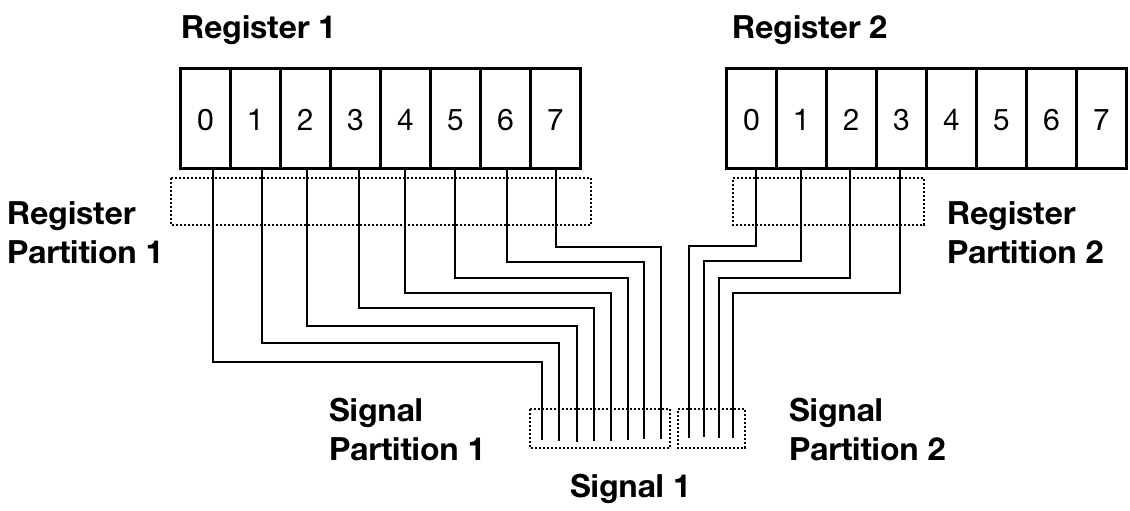
\includegraphics[width = \textwidth]{signalregisterpartitions}
\caption{Mappings of Signal-Register Partitions\label{fig:Mappings of Signal-Register Partitions}}
\end{figure}

Therefore, we designed UI for two cases shown in Figure \ref{fig:Editor UI for Multi-bit Signals} and \ref{fig:Editor UI for Single-bit Signals}. In case of a single-bit signal, users just need to select a certain register and a certain bit of it to map the signal to. Users don't have to explicitly add a signal-register mapping to the partition list. In case of a multi-bit signal, however, users must determine the signal partition by giving its MSB and LSB, select a register, and a register partition. Then, add the signal-register partition to the candidate list. Of course, users can also remove signal-register mapping from the list. To make it more user friendly, we can add a new register by clicking on the button beside the register combo box.  

\begin{figure}[htb]
\centering
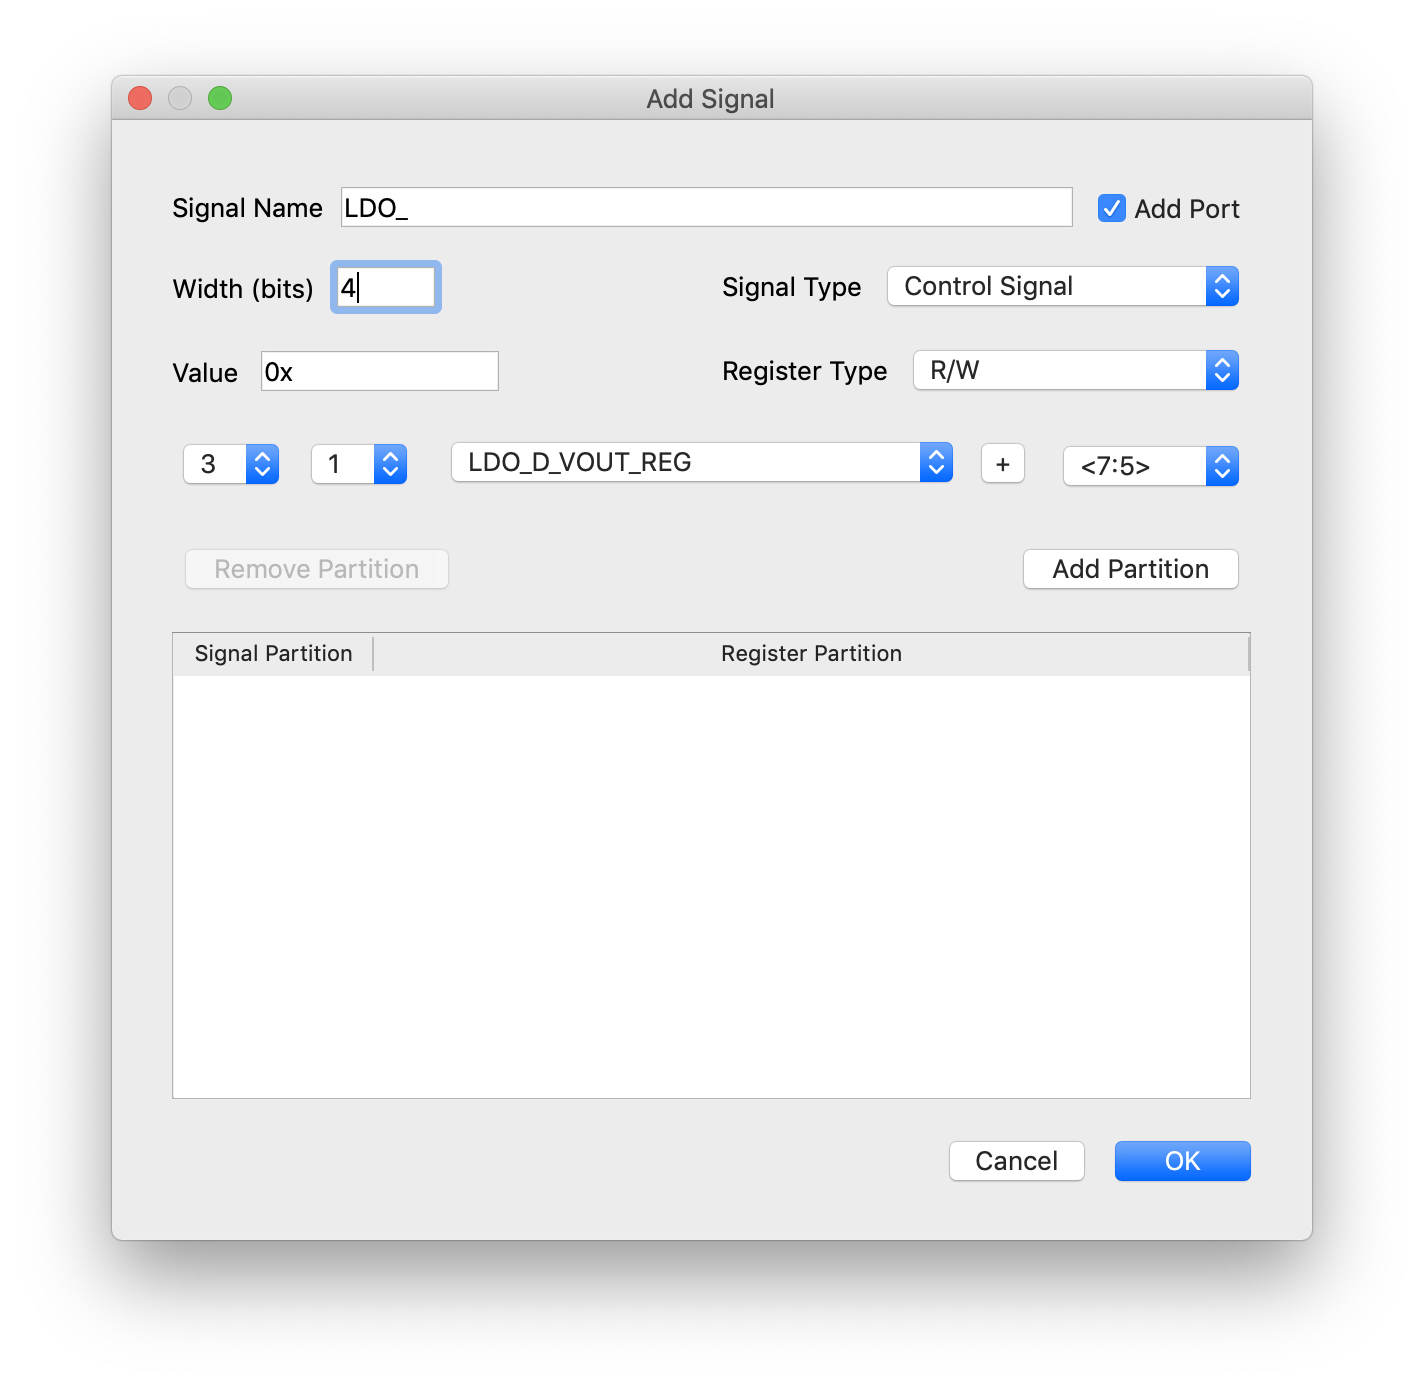
\includegraphics[width = 0.8 \textwidth]{multibitsignal}
\caption{Editor UI for Multi-bit Signals\label{fig:Editor UI for Multi-bit Signals}}
\end{figure}

\begin{figure}[htb]
\centering
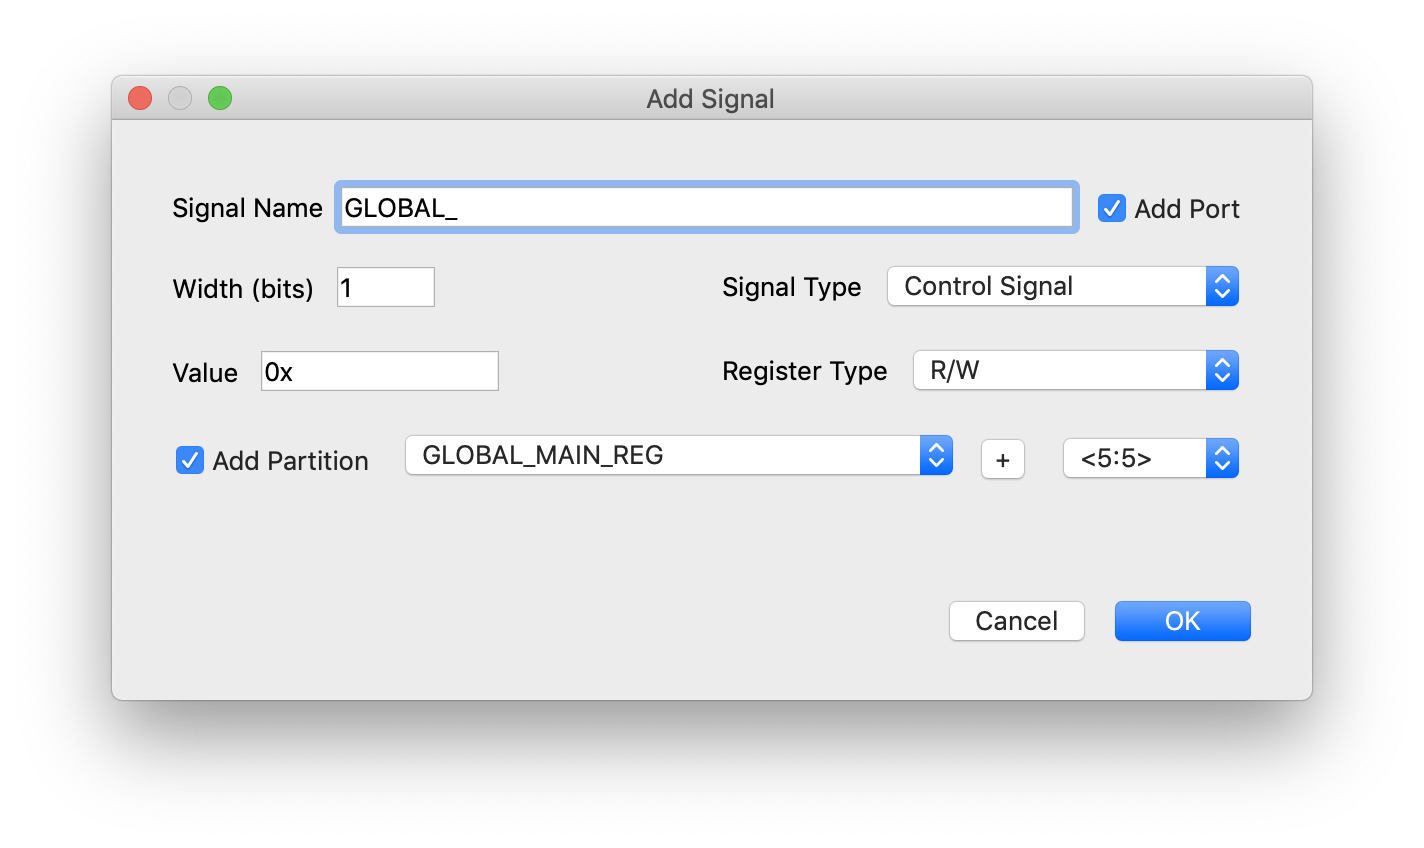
\includegraphics[width = 0.8 \textwidth]{singlebitsignal}
\caption{Editor UI for Single-bit Signalsl\label{fig:Editor UI for Single-bit Signals}}
\end{figure}

Widgets in the \textbf{EditSignalDialog} have pretty strong interaction with each other. Whenever the signal width changes, the signal-register mappings might be invalid, thus we have to clear the candidate list. Also, we have to adjust the UI according to the signal width. If the signal type changes, we have to retrieve from the database the register types available for this signal type, and change the items in the register type combo box. If the current register type changes, we have to clear the signal-register mapping candidate list, and retrieve registers of such type from the database. Whenever the candidate list changes, we also have to find available signal partitions. It is crucial that a signal bit cannot be mapped to more than one register bit, and the other way around. The register partition combo box changes according to the signal LSB and MSB combo boxes. The signal/slot technique provided by Qt makes these changes much more tractable.

The \textbf{EditDocumentDialog} allows users to add document items to the current item in the \textbf{ChipNavigator}, or edit existing ones. It is named after \textbf{dialog} but it is actually not, because we want to incorporate it in the \textbf{DocumentEditorView}, and this is not possible for a dialog. Instead, it is a subclass of \textbf{QWidget}. However, we designed it following the the pattern of the editor dialogs.

We defined three document types, text, image and table. Thus, the \textbf{EditDocumentDialog} was designed so that it can take in all document types. To make this possible the dialog has a stacked widget containing three pages, each handling a specific document type. In the previous section the \textbf{DocumentEditorView} example in Figure \ref{fig:Document Editor View} has already shown the page for text documents. The image page and the table page are shown in Figure \ref{fig:Image Document} and \ref{fig:Table Document} respectively.

\begin{figure}[htbp]
\centering
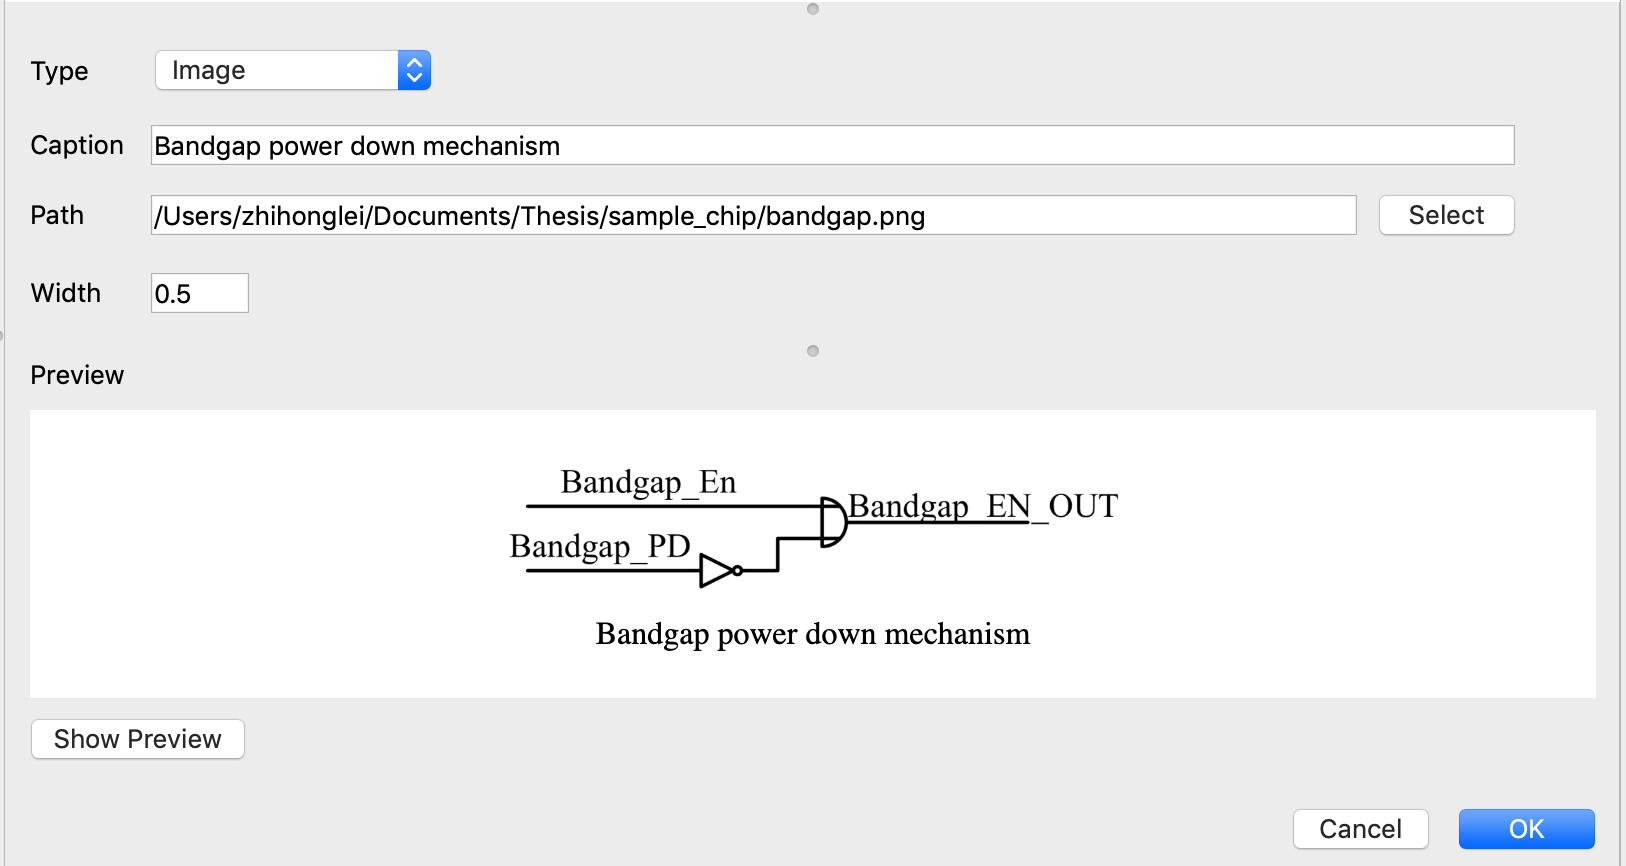
\includegraphics[width = \textwidth]{imagedoc}
\caption{Image Document\label{fig:Image Document}}
\end{figure}

\begin{figure}[htbp]
\centering
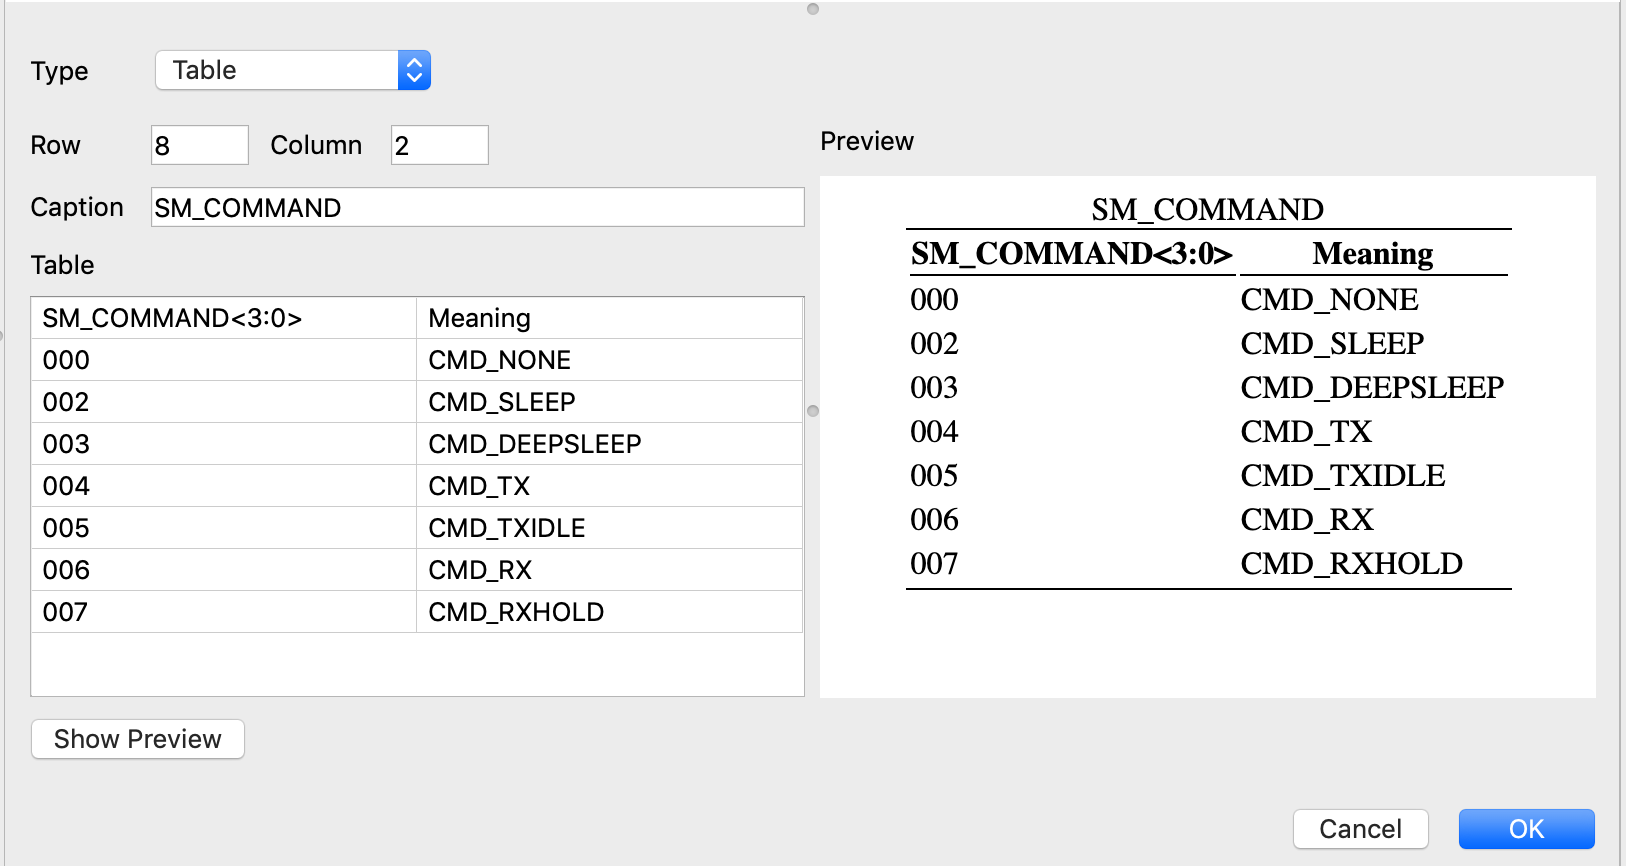
\includegraphics[width = \textwidth]{tabledoc}
\caption{Table Document\label{fig:Table Document}}
\end{figure}

The text page has a \textbf{QPlainTextEdit}, in which we can edit multiple lines of texts. In the image page, we can select an image in a \textbf{QFileDialog}, get its path and specify a caption. It is also important to specify how large the image is in terms of the page width. The number can vary between 0 and 1. In the table page, a \textbf{QLineEdit} holds the caption of the table. The \textbf{QTableWidget} allows users to edit the table contents conveniently. We can specify the number of rows and columns for the table.

We will store the document in the database. The question is how to deal with different types of documents. The text document is simple. We just store the text in the database. For image documents, our solution is to concatenate the caption, width, and the path with a special delimiter, and store the concatenated string in the database. Similarly, for the table documents, we concatenate the caption, row count, column count, and all cell contents. In this solution, of course the image caption, table caption and cell contents must not contain the delimiter. It would be a good idea to use a very rare string as the delimiter. We can easily restore the documents in a reverse way.

It is inevitable that we might have to include math equations in LaTeX format in the documents. In this case, of course we can type LaTeX code "blindly". It would be very nice if we have a preview of the LaTeX math equations. In this way, the input is more visual, and we can check if the code is correct. We also want to have a preview of the table and image. It is important that table cell contents can also contain LaTeX math equations.

To implement the preview, we might want to compile the LaTeX source code to generate a PDF document. Then, we must find a way to display the PDF document in our software. This is not a good idea. First, users have to install a LaTeX compiler on their machines and it must be accessible to the software. Second, Qt does not have a PDF render. We were able to find third-party renders, but they are either of low quality or hard to incorporate in our software.

However, we found MathJax \cite{mathjax}, a JavaScript display engine for mathematics that works in web browsers. With MathJax included in the HTML web page, LaTeX source code can be simply inserted in the HTML code, and browsers can render it properly. We use MathJax with the template in Code \ref{lst:HTML Template for MathJax Render}.

\begin{lstlisting}[language=HTML, caption={HTML Template for MathJax Render\label{lst:HTML Template for MathJax Render}}]
<!-- HTML template -->
<html>
<head>
    <script type="text/x-mathjax-config"> MathJax.Hub.Config({
        tex2jax: {inlineMath: [['$','$'], ['\\(', '\\)']]}});</script>
    <script type="text/javascript" src="MATHJAX_ROOT/MathJax.js"></script>
</head>
<body>
HTML_CONTENT    <!-- write your HTML code here -->
</body>
</html>
\end{lstlisting}

Inspired by this, we can display text, image and table documents in a web browser. For text documents it is quite simple. We just replace \textbf{HTML\_CONTENT} in the HTML template with the text in the text editor. For image and table documents, we created a template respectively, see Code \ref{lst:HTML Template for Images} and \ref{lst:HTML Template for Tables}. Using the image or table template, we generate image or table HTML source code, and replace \textbf{HTML\_CONTENT} in the HTML template.

\begin{lstlisting}[language=html, caption={HTML Template for Images\label{lst:HTML Template for Images}}]
<!-- HTML image template -->
<style>
    figure img {display: block; margin-left: auto; margin-right: auto;}
    figure figcaption { text-align: center;}
</style>
<center>
<figure>
   <img style='width: WIDTH; object-fit: contain' src="IMAGE" alt="CAPTION"/>
    CAPTION
</figure>
</center>
\end{lstlisting}

\begin{lstlisting}[language=html, caption={HTML Template for Tables\label{lst:HTML Template for Tables}}]
<!-- HTML table template -->
<style>
    table {border-top: 1px solid black; border-bottom: 1px solid black}
    th {border-bottom: 1px solid black}
    caption#tab {caption-side: CAPTION_POS}
</style>
<center>
<table>
TABLE
</table>
</center>
\end{lstlisting}

Fortunately, Qt provides a web engine \cite{qtwebengine} based on Chromium \cite{chromium}. Thus, we were able to make a preview based on the web engine. The preview is intrinsically a web browser. To display documents of any types, we generate the HTML source code and fill it into the browser. In this way, the document editor can display the real time preview of the text users are editing.

Another effort we made is to implement an auto-completer. This is especially useful for editing texts. The completer we designed takes all system block names, system block abbreviations, register names and signal names as candidates. Besides these, the software allows users to extend the word list by simply add txt files containing candidate words to the \textbf{completion} directory under the root directory of the software. Figure \ref{fig:Document Completer} shows an example of auto-completion on the text document. We also implemented auto-complement for captions and table cell contents. 

\begin{figure}[htb]
\centering
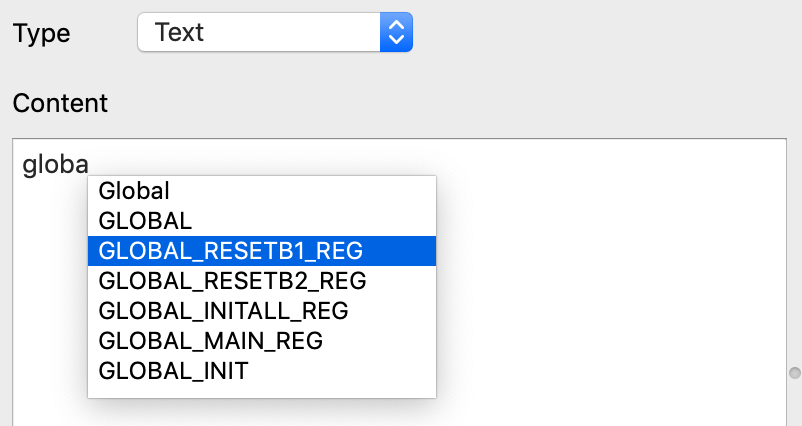
\includegraphics[width = 0.5\textwidth]{completer}
\caption{Document Completer\label{fig:Document Completer}}
\end{figure} 

\section{User Account, Authentication and Password}
For data security reasons, the software is required to provide user access control and authentication. User access control has two levels, the software or database level and the project level. If a user account is created, the user can log in to the software with this account. However, it does not necessarily mean he or she has access to a certain chip project. This is controlled by the project level permissions.

All users must have access to the database, thus, we need to establish database accounts for them. MySQL provides a very good user account management. We can grant different permissions for different users. However, the permissions we want to implement are more complex. For example, in a certain table, a user might have access to row A but not to row B. This is not possible with MySQL. Thus, we have to manage permissions using our software. Against this background, we distinguished the \textit{software} account and \textit{database} account. We store \textit{software} accounts in the database. Users log in to the database using a shared \textit{database} account, retrieve the \textit{software} account information and determine if they have access to the software. Chip designers, database level and project level permissions are also stored in the database.

We defined different database permissions allowing users to add or remove users or projects. A special permission is reserved for the database/software admins, so they have full access to all projects. This means that they can do anything on any projects, even if they are not in the designer list of those projects. We predefined two database roles, the admin and the standard user. However, we can extend the database roles without modifying the software. Similarly, we defined different project permissions allowing chip designers to add system blocks, remove the system blocks they are in charge of, read all system blocks, add or remove chip designers. An implicit permission is that designers can always edit the system blocks they are responsible for.

To make use of the database and project permissions, we designed an \textbf{Authenticator} class as in Code \ref{lst:Definition of the Authenticator}. To make block level authentication more manageable, we also defined block permissions here. They are determined by project permissions and whether the user is the responsible person of the system block. The \textbf{Authenticator} class allows users to set database permissions, project permissions and block permissions. The permissions are stored in member variables \textbf{db\_permissions\_}, \textbf{project\_permissions\_}, \textbf{block\_permissions\_} of data type \textbf{int}. Each bit of the permissions variables represents a specific permission, which is defined in the enumeration \textbf{DATABASE\_PERMISSIONS}, \textbf{PROJECT\_PERMISSIONS}, and \textbf{BLOCK\_PERMISSIONS}. We set or retrieve permissions using bit operations. For example, to set the \textbf{ADD\_USER} permission, we make the 0th bit of \textbf{db\_permissions\_} be 1. To retrieve the \textbf{ADD\_USER} permission, we get the value of the 0th bit of \textbf{db\_permissions\_}.

\begin{lstlisting}[language=C++, caption={Definition of the Authenticator\label{lst:Definition of the Authenticator}}]
class Authenticator
{
public:
    enum DATABASE_PERMISSIONS
    {
        ADD_USER = 1 << 0,
        // ...
        FULL_ACCESS_TO_ALL_PROJECTS = 1 << 4
    };
    // enum PROJECT_PERMISSIONS
    // enum BLOCK_PERMISSIONS
    
    Authenticator(const QString& db_role_id, const QString& project_role_id);
    Authenticator();

    void set_database_permissions(const QString& db_role_id);
    void set_project_permissions(const QString& project_role_id);
    void set_project_permissions(bool setting);
    void set_block_permissions(bool setting);
    void freeze(bool frozen=true);

    // database permissions
    bool can_add_user() const;
    // ...
    bool can_fully_access_all_projects() const;

    // project permissions
    bool can_add_block() const;
    // ...
    bool can_fully_access_all_blocks() const;
    
    // block permissions
    bool can_add_signal() const;
    // ...
    bool can_edit_document() const;
    
    bool frozen() const;

    void clear_database_permission();
    void clear_project_permission();
    void clear_block_permission();
    void clear_all_permission();

private:
    int db_permissions_ = 0, project_permissions_ = 0, block_permissions_;
    bool frozen_;
};
\end{lstlisting}

We provide a convenient way for managing user accounts using the \textbf{UserManagementDialog}. It allows database admins to add or remove users. To add a user, we need a \textbf{CreateUserDialog}. The username and initial password are specified and a database role is selected. Like the editor dialogs, the \textbf{CreateUserDialog} has to check whether the username is valid. After creation of a user account, users can then log in to the software using the account with the initial password. Users can change their passwords easily using the \textbf{ChangePasswordDialog}. To remove a user, however, will be tricky. The users to be deleted might be the owner of some chips. They might be a designer in some chips, and responsible for some system blocks. In this case, our solution is to replace the users in those chips with the database admin who is deleting these users.

On the project level, designers can be added to a chip with the \textbf{EditChipDesignerDialog}, where a user and a project role are selected. Before adding a designer, the dialog shall check whether the selected user already exists in the current project. We can also delete a chip designer. Like removing a user, the software has to replace the designers in this project with a project admin.

As previously described, the software account and database account are not the same. In our solution, all software users share a single database account. The problem is that we don't want users to know the password to the database to prevent them from bypassing the software and directly work on the database. This might cause serious data security problems.

Our solution is to introduce an encryptor and decryptor. We designed an encryption class using the AES algorithm \cite{daemen2013design}. The encryptor can encrypt a plain password with a key. With this key and encrypted password, the decryptor can generate the original plain password. Only the admins know the password. They generate encrypted password, and give users the key and the encrypted password instead of the original password. We made a tool for admins to make encrypted passwords easily as shown in Figure \ref{fig:Encryptor Dialog}.

\begin{figure}[htb]
\centering
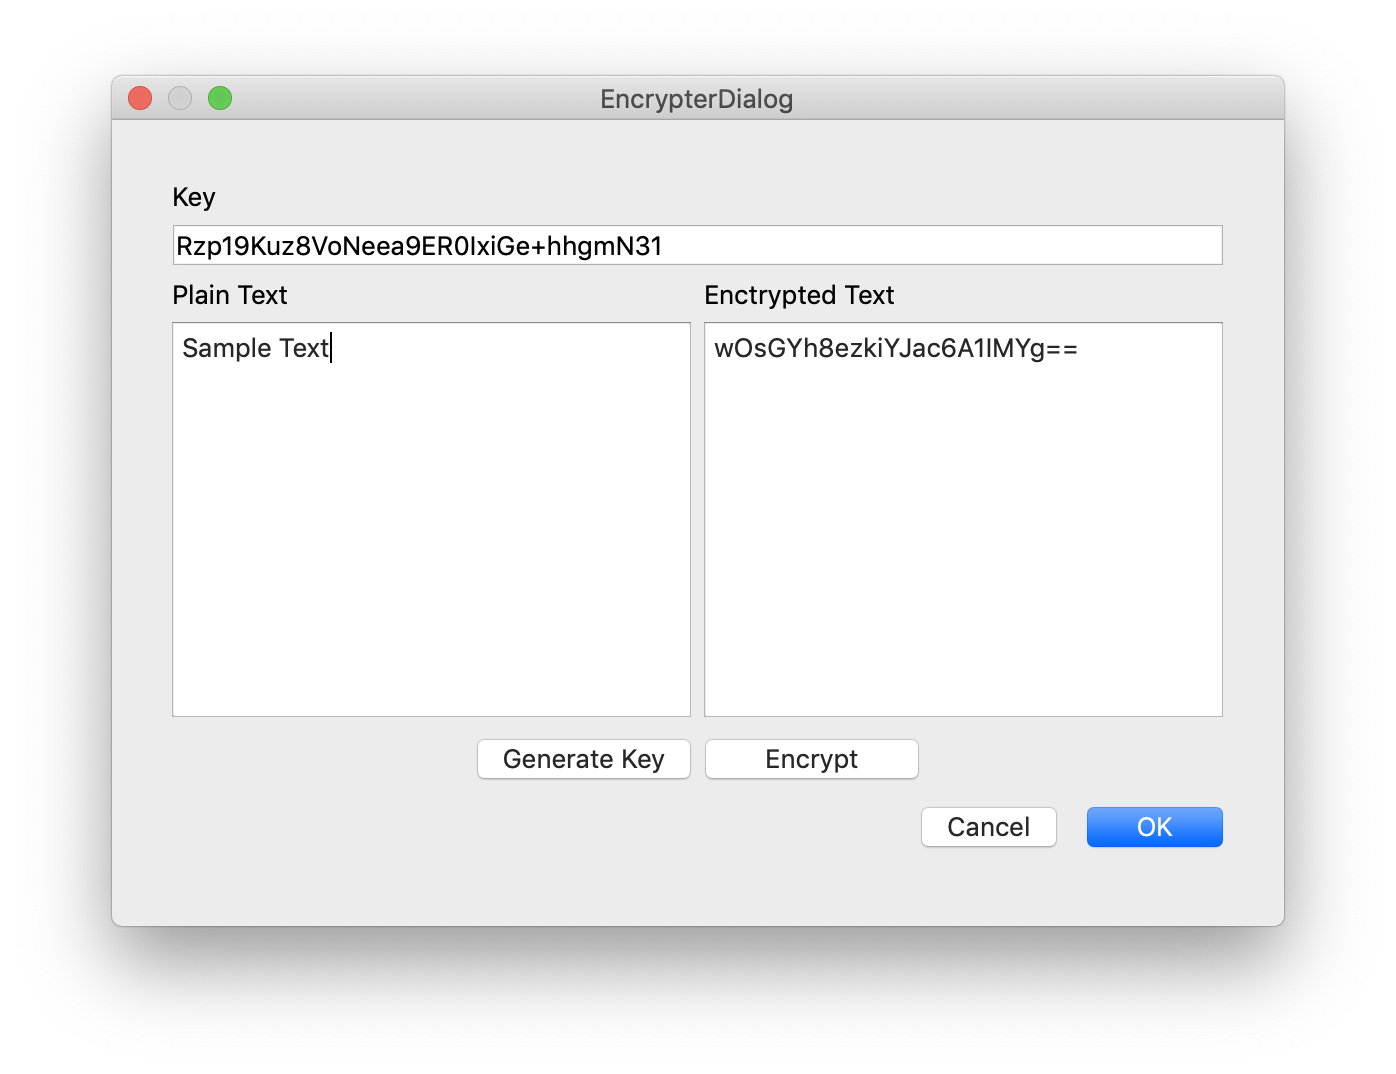
\includegraphics[width = 0.8\textwidth]{encryptor}
\caption{Encryptor Dialog\label{fig:Encryptor Dialog}}
\end{figure} 

\section{Signal and Register Naming}
In practice, we name signals and registers after a certain pattern. For example, a register might be named after \textbf{\$\{BLOCK\_ABBREVIATION\}\_MAIN\_REG}. In this example, the block abbreviation is prepended to the central name \textbf{MAIN}, and a constant string \textbf{REG} is appended to the name. The block abbreviation, what we call the given name, and the suffix \textbf{REG} are concatenated with an underscore.

The problem is that, if we have to change a system block's abbreviation, then all registers have to be renamed. This leads to more database operations and unreliability. Our solution is simple: we only store the given name in the database. However, the extended name is generated with the naming template and the given name. 

Thus, we designed a \textbf{NamingTemplate} class to generate the extended name with the given name, and the other way around. The idea is that we maintain a naming template like \textbf{\$\{BLOCK\_ABBREVIATION\}\_\$\{GIVEN\_NAME\}\_REG}. The naming template contains variables like \textbf{\$\{Variable\}} and constants. The \textbf{\$\{GIVEN\_NAME\}} variable must always be in the template. In this example, to generate the extended name, we simply replace the variables with the abbreviation name of the current system block, and the given name of the current register, which is retrieved from the database. Similarly, we can also extract the given name given an extended name.

\begin{figure}[htb]
\centering
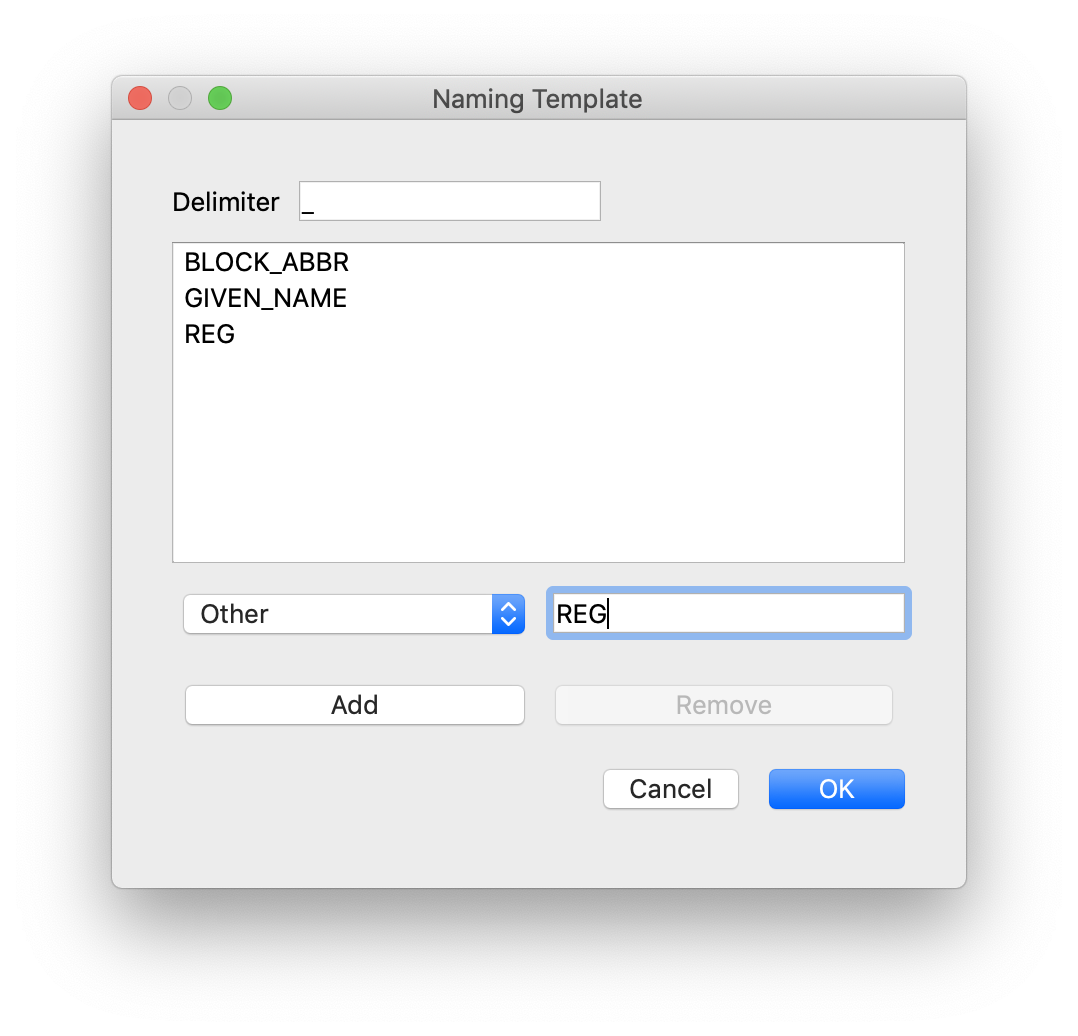
\includegraphics[width = 0.7\textwidth]{namingtemplatedialog}
\caption{Naming Template Dialog\label{fig:Naming Template Dialog}}
\end{figure} 

To change the naming of signals or registers, we don't have to do anything on the database. We simply make a new naming template and refresh the UI. We designed a very friendly dialog in Figure \ref{fig:Naming Template Dialog} to change the naming template. Users just need to add keywords or constants, and specify a delimiter.

\section{SPI Interface Generation}
With all the chip definitions and document items, our final goals are generating the SPI configuration interface and a LaTeX documentation. We might want to generate the interface in different languages later, but so far we only implemented VHDL. Despite of this, during design and implementation, we already left flexibility for extensions.

The VHDL SPI interface consists of two files, the interface package in which basic information about the chip is defined, and the interface in which the VHDL interface and behavior are defined. Code \ref{lst:VHDL Package Template} and Code \ref{lst:VHDL Interface Template} are an example of the package and interface templates. Users can define a package and an interface template with predefined markers. The software will replace the markers with what it generates from the database.

\begin{lstlisting}[language=VHDL, caption={VHDL Package Template\label{lst:VHDL Package Template}}]
-- sample VHDL package template
LIBRARY ieee;
  USE ieee.std_logic_1164.all;
  USE ieee.numeric_std.all;
  
PACKAGE interface_package IS

  constant address_width      : integer := 12;
  constant byte_size          : integer := 8;
  constant reg_width           : integer := 8;
  -- FIFO
  constant byte_counter_width : integer := 10;
  constant fifo_size          : integer := 2**byte_counter_width;
  constant packet_size        : integer := 2**byte_size;

   -- REGISTER ADDRESSES
  @PACKAGE_ADDRESSES    -- to be completed by EDA tool

  -- REGISTER_INITIAL VALUES
  @PACKAGE_INITS    -- to be completed by EDA tool
  
END PACKAGE interface_package;
\end{lstlisting}

In the package template there are two makers, one for register address definitions, and the other for initial values definitions for writable registers. Since we allocated each system block a start address, it's easy to infer the address for each register. The initial values of each writable registers are not straightforward. We have to compute initial values for each register bit by looking for the corresponding signal bit it is mapped to, and the initial signal value. Then, the initial values of the registers are obtained by concatenating the initial values of each register bit.

\begin{lstlisting}[language=VHDL, caption={VHDL Interface Template\label{lst:VHDL Interface Template}}]
-- sample VHDL package template
library IEEE;
use IEEE.STD_LOGIC_1164.ALL;
use IEEE.NUMERIC_STD.ALL;

LIBRARY work;
use work.interface_package.ALL;

entity interface is
  generic
  (
    data_width : integer := 12
  );
  port
  (
    resetn                    : in  std_logic;
    clk_main                  : in  std_logic;
    enable                    : in  std_logic;
    
    -- REGISTER SIGNAL PORT DEFINITIONS      
    @PORT_DEFINITIONS
 
  );
end interface;

architecture Behavioral of interface is

  -- INTERNAL SIGNALS FOR INTERFACE FUNCTION
  signal addr_buffer            : std_logic_vector(address_width-1 downto 0);
  signal reg_read_buffer        : std_logic_vector(byte_size-1 downto 0);
  signal byte_ext2asc           : std_logic_vector(byte_size-1 downto 0);
  
  -- INTERNAL SIGNALS NOT CREATED BY THE AUTOMATIC EXPORT
  signal SM_INVERT_FIFO_CLK     : std_logic;  
  signal SM_FIFO_SPI_RESETB     : std_logic;
  signal CHIP_ID_VALUE		: std_logic_vector(16-1 downto 0);
  signal CHIP_REGPAGE_CTRL	: std_logic_vector(2-1 downto 0);

  -- REGISTER DEFINITIONS
  @REGISTER_DEFINITIONS

begin 
  
  reg_write_proc: PROCESS(clk_main, resetn, enable)
  BEGIN
    if resetn = '0' then
      -- Registers
      @REGISTER_INIT

      new_spi_reg_write       <= '0';
    else
      if rising_edge(clk_main) and enable = '1' then
        if current_state = S_DATW and byte_ext2asc_rising = '1' then
          new_spi_reg_write  <= '1';
          case addr_buffer is
            @REG_WRITE_ACCESS

            when others                         => null;
          end case;
        else
          new_spi_reg_write <= '0';
        end if;
      end if;
    end if;
  END PROCESS reg_write_proc;
  
  reg_read_proc: PROCESS(clk_main, resetn, enable)
  BEGIN
    if resetn = '0' then
      reg_read_buffer  <= (others => '0');
      new_spi_reg_read            <= '0';
    else
      if rising_edge(clk_main) and enable = '1' then
        if current_state = S_DATR then
          new_spi_reg_read        <= '1';
          case addr_buffer is
            @REG_READ_ACCESS

            when others                         => null;
          end case;
        else 
          new_spi_reg_read        <= '0';
          reg_read_buffer         <= (others => '0');
        end if;
      end if;
    end if;
  END PROCESS reg_read_proc;
  
  @SIGNAL_ASSIGNMENTS
  
end Behavioral;
\end{lstlisting}

The interface is more complex. It consists of two code blocks, the entity definition, and the behavioral definition. In the entity definition, the software shall complete the port definitions. All port signals should be included. Then, in the behavioral definition, the software first completes the register definitions. Then, it should complete the read and write procedure. In the reading procedure, data is read from external and written to a certain register according to the address buffer. In the write procedure, data is read from a certain register and written to external. Finally, the software should assign values to signals or registers. In case of a read-only register, the software shall assign to it values from the signals it is mapped to. In case of a writable register, the software shall assign values to the signals it is mapped to. Paged registers are dealt with in a special way.

We designed a \textbf{VHDLGenerator} class. The generation procedure of the interface is described with the Code \ref{lst:Logic of VHDL Interface Generation}. Generation of the package follows the same structure.

\begin{lstlisting}[language=C++, caption={Logic of VHDL Interface Generation\label{lst:Logic of VHDL Interface Generation}}]
// vhdl_generator.h
QString VHDLGenerator::generate_interface() const
{
    QString ports,
            register_definitions, register_inits,
            register_write_accesses, register_read_accesses,
            readonly_register_assignments,
            control_signal_assignments,
            paged_register_assignments;
            
    QVector<QString> blocks = read_system_blocks();
    for (const auto& block : blocks)
    {
        QVector<QString> interface_block = generate_interface_block(block);
        ports += interface_block[0];
        register_definitions += interface_block[1];
        register_inits += interface_block[2];
        register_write_accesses += interface_block[3];
        register_read_accesses += interface_block[4];
        readonly_register_assignments += interface_block[5];
        control_signal_assignments += interface_block[6];
        paged_register_assignments += interface_block[7];
    }
    QString interface = get_interface_template();
    interface.replace(marker_ports, ports);
    interface.replace(marker_register_definitions, register_definitions);
    interface.replace(marker_register_init, register_inits);
    interface.replace(marker_register_write, register_write_accesses);
    interface.replace(marker_register_read, register_read_accesse);
    interface.replace(marker_signal_assignment, signal_assignments);
      
    return interface;
}

QVector<QString> VHDLGenerator::generate_interface_block(block) const
{
    QVector<QString> signals = read_signals(block);
    QVector<QString> registers = read_registers(block);
    QString ports,
            register_definitions, register_inits,
            register_write_accesses, register_read_accesses,
            readonly_register_assignments, 
            control_signal_assignments, 
            paged_register_assignments;
            
    for (const auto& register : registers)
    {
        register_definitions += generate_register_definition(register);
        register_read_accesses += generate_reading_register(register);
        if (writable(register))
        {
            register_inits += generate_initializing_register(register);
            register_write_accesses += generate_writing_register(register);
        }
        else
        {
            readonly_register_assignments += generate_assigning_value_to_readonly_register(register);
        }
        if (paged_register(register))
            paged_register_assignments += generate_assigning_value_to_paged_register(register);
    }
    
    for (const auto& signal : signals)
    {
        if (port_signal(signal)) 
            ports += generate_port_definition(signal);
        if (control_signal(signal)) 
            control_signal_assignments += generate_assigning_value_to_constrol_signal(signal);
    }
    
    return {ports,
            register_definitions, register_inits,
            register_write_accesses, register_read_accesses,
            readonly_register_assignments, 
            control_signal_assignments, 
            paged_register_assignments};
}
\end{lstlisting}

We made a \textbf{SPIGenerationDialog} class for users to configure the export. See Figure \ref{fig:SPI Generation Dialog}. The design pattern is similar to the previous editor dialogs. Since the generated code must be directly usable, we have to make sure there are no errors. Sanity checks must be done.

\begin{figure}[htb]
\centering
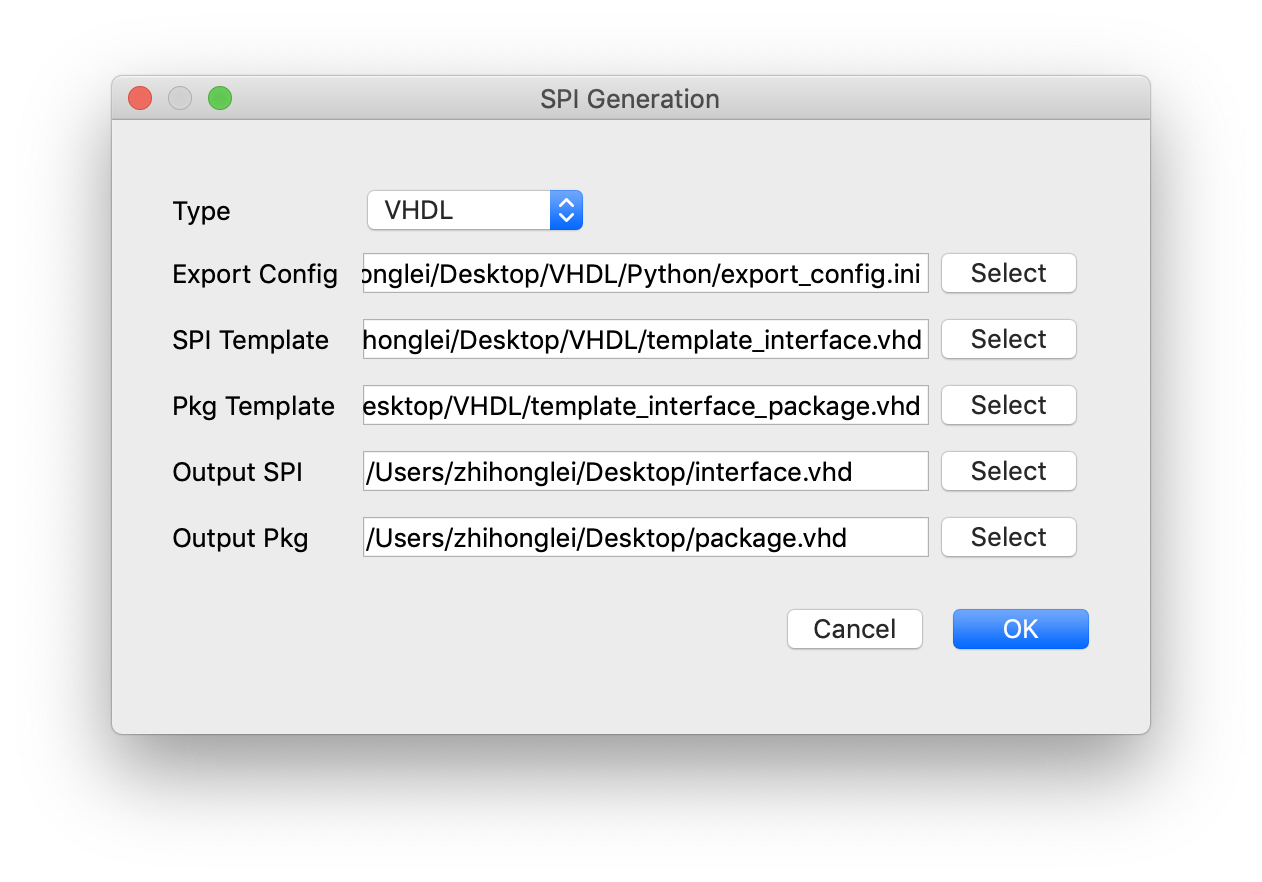
\includegraphics[width = 0.8\textwidth]{spigenerationdialog}
\caption{SPI Generation Dialog\label{fig:SPI Generation Dialog}}
\end{figure} 

\section{Document Generation\label{sec:Document Generation}}
So far chip designers have added documents to each system block, register and signal, and also the chip itself as well. The software will compose them and generate a complete documentation.

The documentation has a good CHIP-BLOCK-REGISTER-SIGNAL structure as in Figure \ref{fig:Structure of the Documentation}. Thus, we designed a \textbf{DocumentGenerator} following this structure. Code \ref{lst:Definition of the Document Generator} shows the definition of the \textbf{DocumentGenerator} class. For simplicity, function parameters and member variables are omitted.

\begin{figure}[htb]
\centering
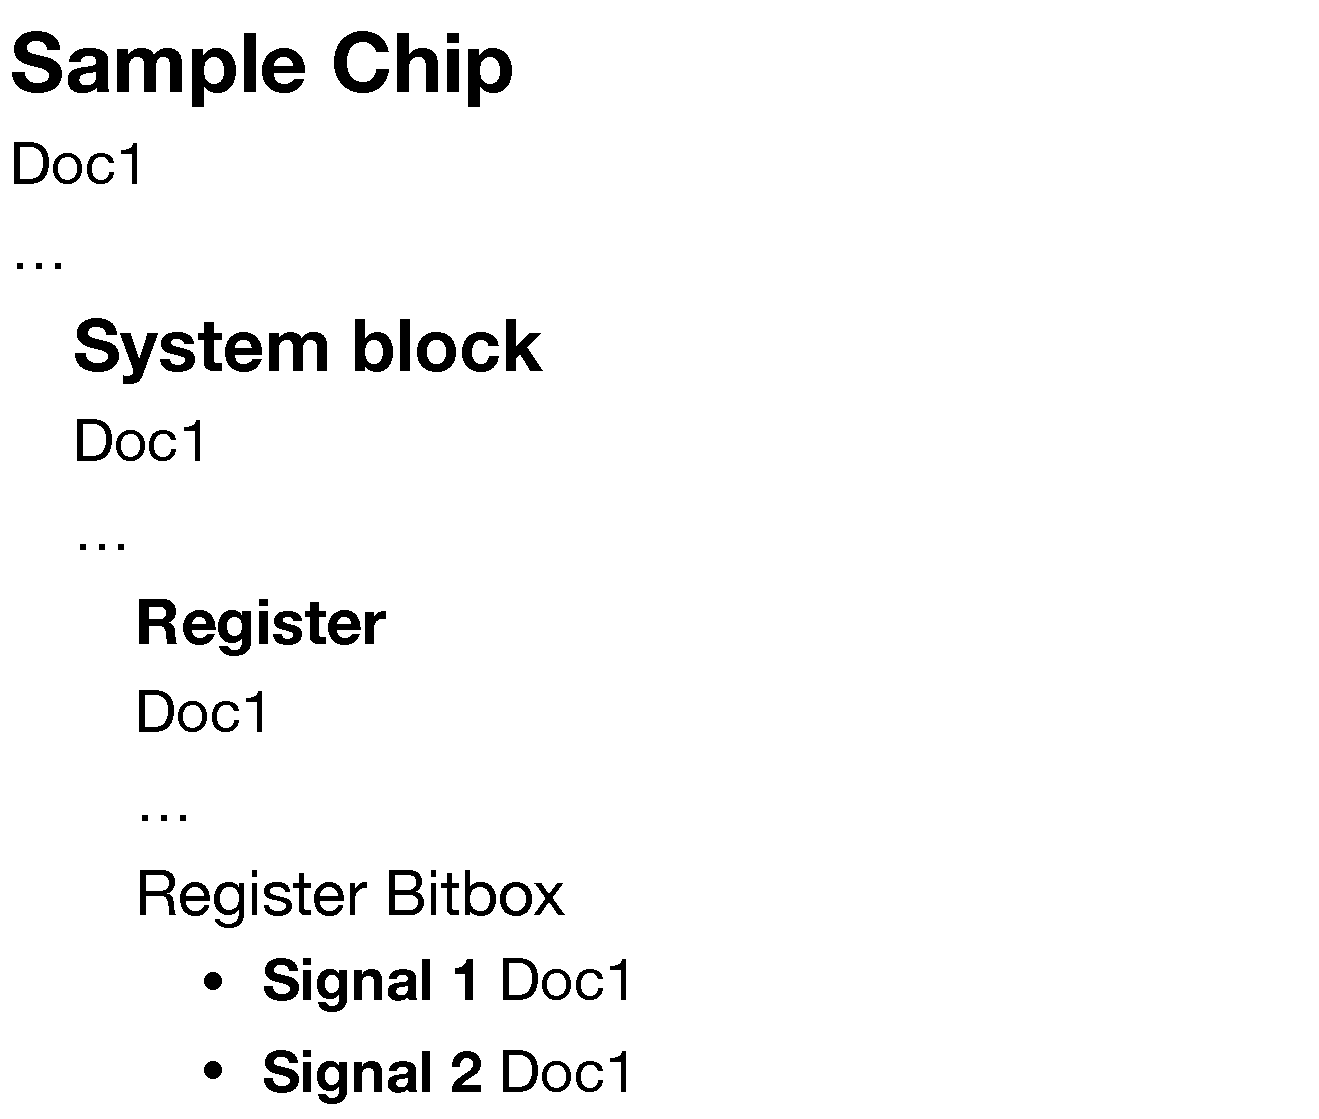
\includegraphics[width = 0.6\textwidth]{docstructure}
\caption{Structure of the Documentation\label{fig:Structure of the Documentation}}
\end{figure} 

\begin{minipage}{\linewidth}
\begin{lstlisting}[language=C++, caption={Definition of the Document Generator\label{lst:Definition of the Document Generator}}]
// document_generator.h

// functions to generate the LaTeX documentation
// parameters are omitted
QString generate_tex_document();
QString generate_chip_level_tex_document();
QString generate_block_level_tex_document();
QString generate_register_level_tex_document();
QString generate_register_bit_table_tex();
QString generate_register_signal_bullets_tex();

// static functions to generate single documents into LaTeX
static QString generate_text_tex(const QString& text);
static QString generate_image_tex(const QString& caption, const QString& width, const QString& path);
static QString generate_table_tex(const QString& caption, const QVector<QVector<QString> >& cells);
\end{lstlisting}
\end{minipage}

In previous sections, we have introduced a document preview for the document editor. It is basically a web browser rendering HTML web pages with LaTeX source code with the help of MathJax. Since the software is already able to display a single document, it is pretty straightforward to implement a function to generate a full documentation in HTML format, and make a preview of the complete documentation based on MathJax and web browsers. Figure \ref{fig:Document Preview in HTML Format} is an example of the documentation preview using our software. In fact, in some cases HTML would be a better choice than LaTeX, for example, if the Chair of IAS wants to create an internal wiki about the ASIC chips.

\begin{figure}[htb]
\centering
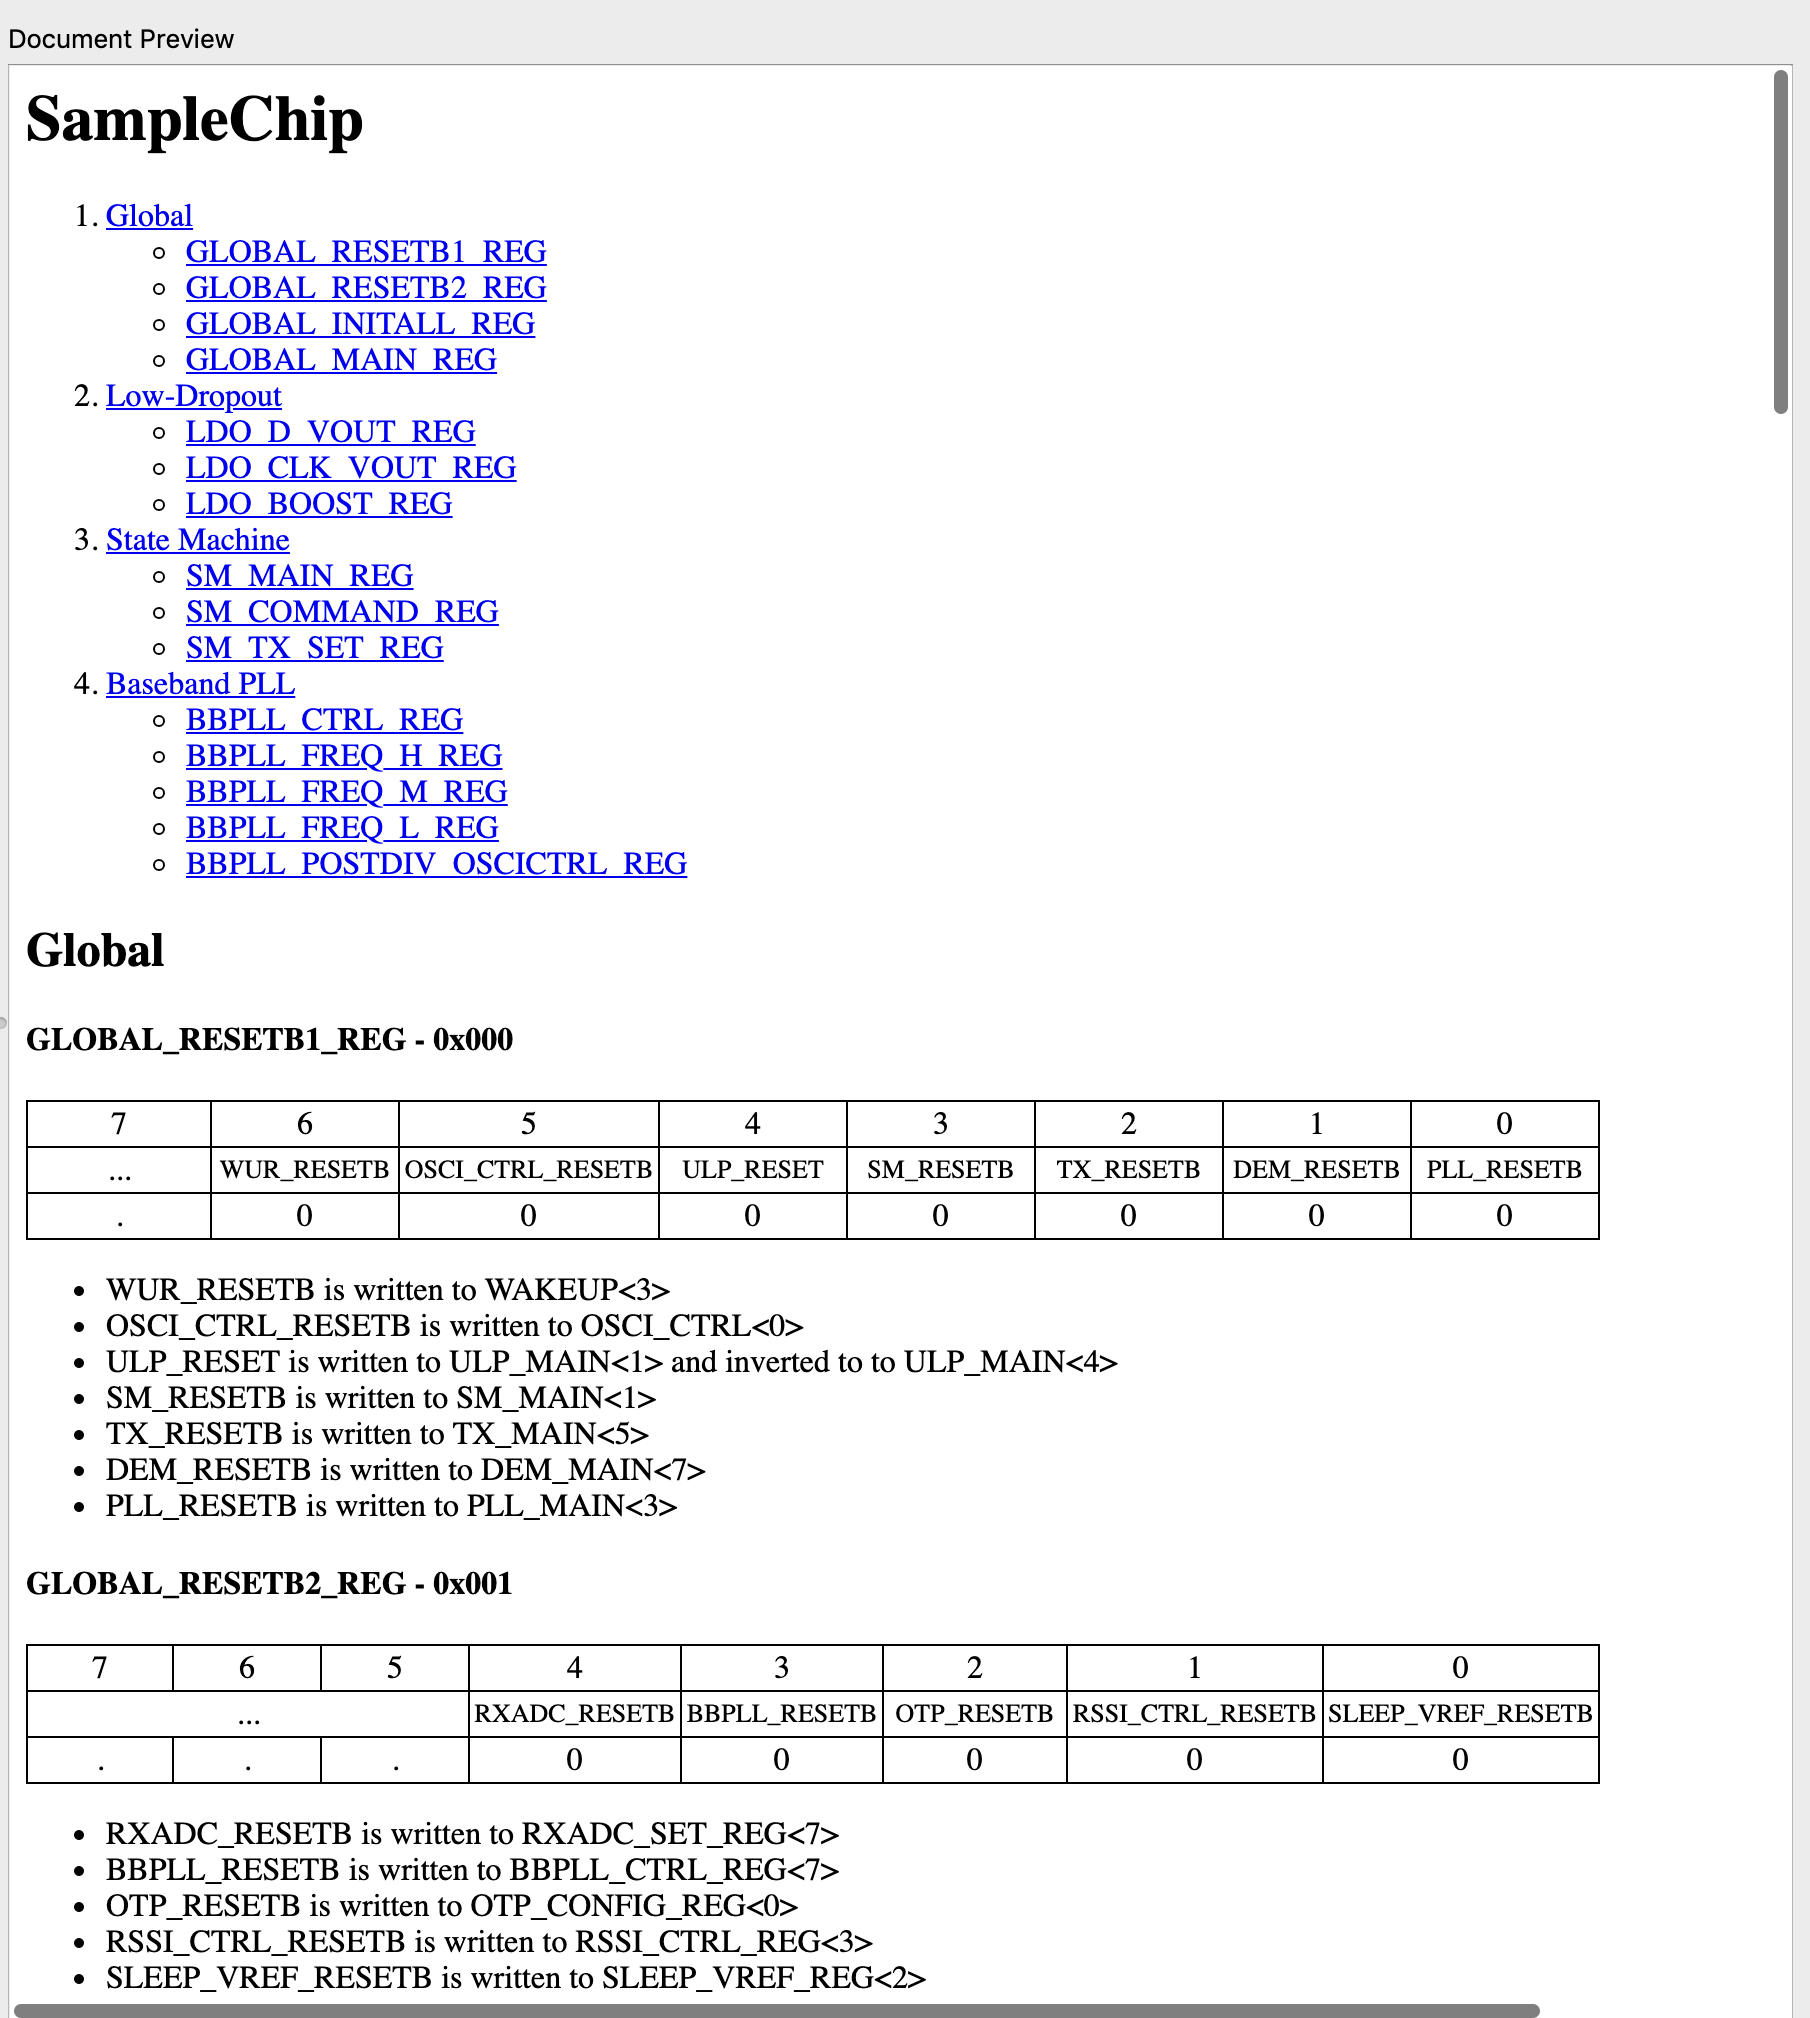
\includegraphics[width = \textwidth]{htmldocexample}
\caption{Document Preview in HTML Format\label{fig:Document Preview in HTML Format}}
\end{figure} 

We created a \textbf{DocumentGenerationDialog} as in Figure \ref{fig:Documentation Generation Dialog} for users to select the document format, configure the documentation and select which system blocks they want to include in the documentation. 

\begin{figure}[htb]
\centering
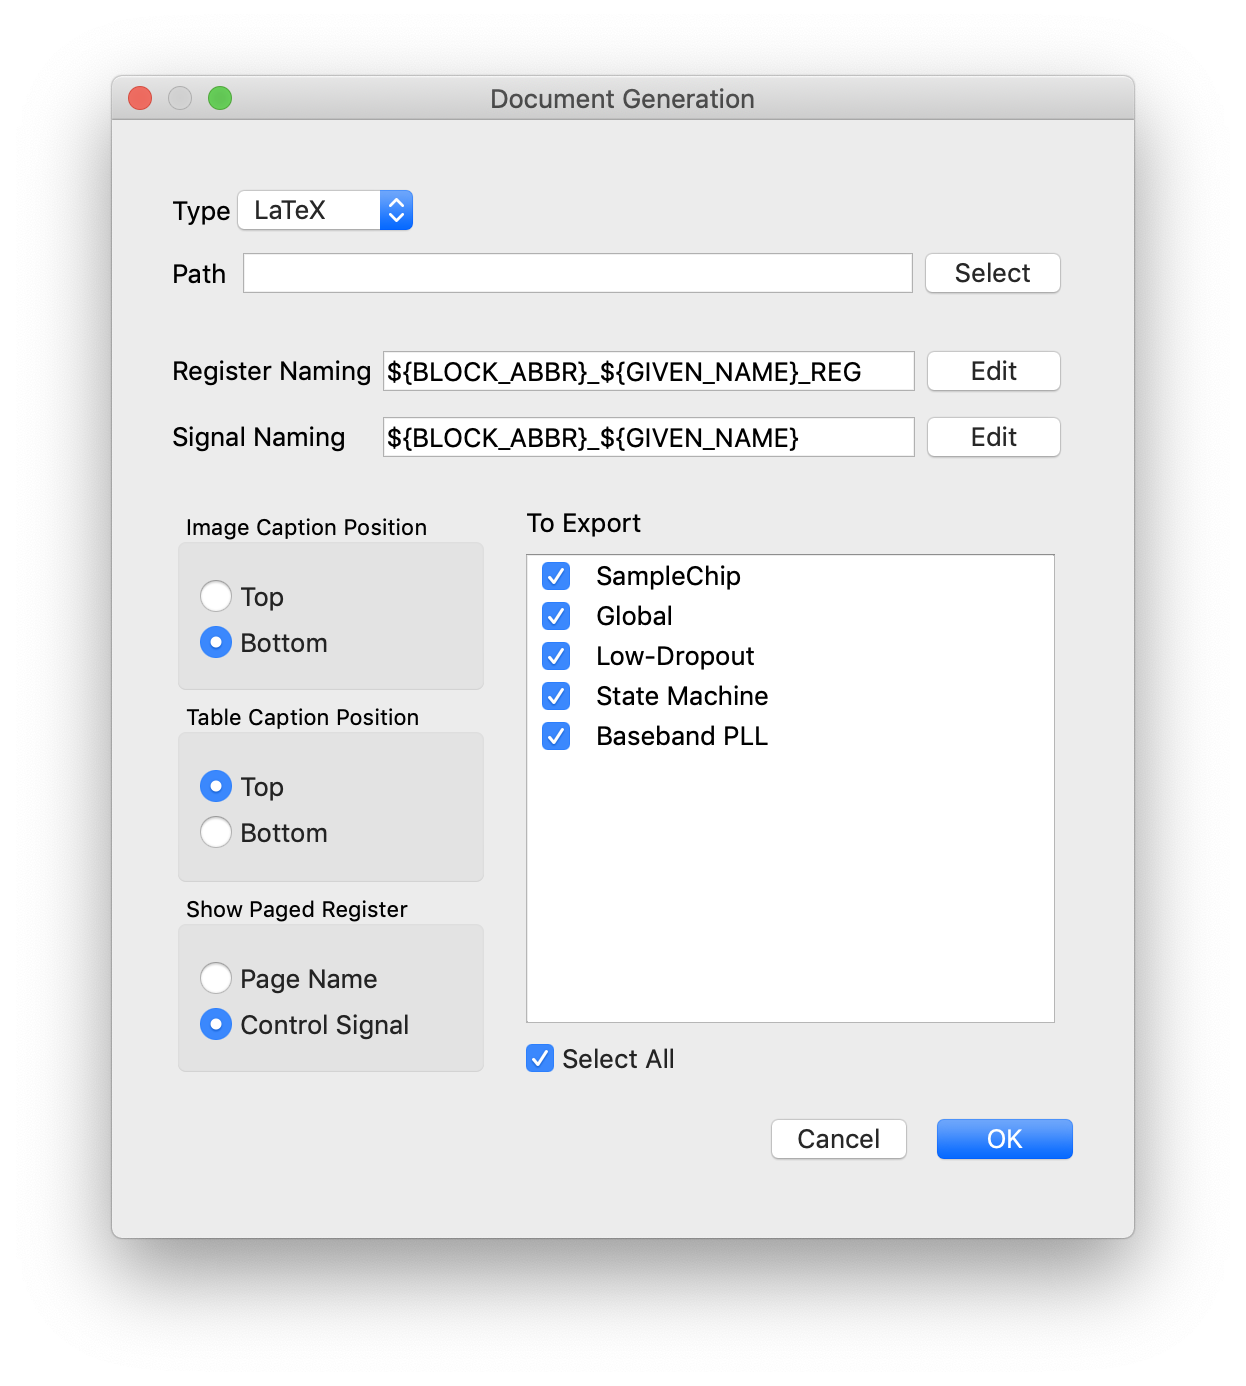
\includegraphics[width = 0.8\textwidth]{docgenerationdialog}
\caption{Documentation Generation Dialog\label{fig:Documentation Generation Dialog}}
\end{figure} 
